% Options for packages loaded elsewhere
\PassOptionsToPackage{unicode}{hyperref}
\PassOptionsToPackage{hyphens}{url}
%
\documentclass[
  oneside]{book}
\usepackage{amsmath,amssymb}
\usepackage{iftex}
\ifPDFTeX
  \usepackage[T1]{fontenc}
  \usepackage[utf8]{inputenc}
  \usepackage{textcomp} % provide euro and other symbols
\else % if luatex or xetex
  \usepackage{unicode-math} % this also loads fontspec
  \defaultfontfeatures{Scale=MatchLowercase}
  \defaultfontfeatures[\rmfamily]{Ligatures=TeX,Scale=1}
\fi
\usepackage{lmodern}
\ifPDFTeX\else
  % xetex/luatex font selection
\fi
% Use upquote if available, for straight quotes in verbatim environments
\IfFileExists{upquote.sty}{\usepackage{upquote}}{}
\IfFileExists{microtype.sty}{% use microtype if available
  \usepackage[]{microtype}
  \UseMicrotypeSet[protrusion]{basicmath} % disable protrusion for tt fonts
}{}
\makeatletter
\@ifundefined{KOMAClassName}{% if non-KOMA class
  \IfFileExists{parskip.sty}{%
    \usepackage{parskip}
  }{% else
    \setlength{\parindent}{0pt}
    \setlength{\parskip}{6pt plus 2pt minus 1pt}}
}{% if KOMA class
  \KOMAoptions{parskip=half}}
\makeatother
\usepackage{xcolor}
\usepackage{longtable,booktabs,array}
\usepackage{calc} % for calculating minipage widths
% Correct order of tables after \paragraph or \subparagraph
\usepackage{etoolbox}
\makeatletter
\patchcmd\longtable{\par}{\if@noskipsec\mbox{}\fi\par}{}{}
\makeatother
% Allow footnotes in longtable head/foot
\IfFileExists{footnotehyper.sty}{\usepackage{footnotehyper}}{\usepackage{footnote}}
\makesavenoteenv{longtable}
\usepackage{graphicx}
\makeatletter
\def\maxwidth{\ifdim\Gin@nat@width>\linewidth\linewidth\else\Gin@nat@width\fi}
\def\maxheight{\ifdim\Gin@nat@height>\textheight\textheight\else\Gin@nat@height\fi}
\makeatother
% Scale images if necessary, so that they will not overflow the page
% margins by default, and it is still possible to overwrite the defaults
% using explicit options in \includegraphics[width, height, ...]{}
\setkeys{Gin}{width=\maxwidth,height=\maxheight,keepaspectratio}
% Set default figure placement to htbp
\makeatletter
\def\fps@figure{htbp}
\makeatother
\setlength{\emergencystretch}{3em} % prevent overfull lines
\providecommand{\tightlist}{%
  \setlength{\itemsep}{0pt}\setlength{\parskip}{0pt}}
\setcounter{secnumdepth}{5}
% definitions for citeproc citations
\NewDocumentCommand\citeproctext{}{}
\NewDocumentCommand\citeproc{mm}{%
  \begingroup\def\citeproctext{#2}\cite{#1}\endgroup}
\makeatletter
 % allow citations to break across lines
 \let\@cite@ofmt\@firstofone
 % avoid brackets around text for \cite:
 \def\@biblabel#1{}
 \def\@cite#1#2{{#1\if@tempswa , #2\fi}}
\makeatother
\newlength{\cslhangindent}
\setlength{\cslhangindent}{1.5em}
\newlength{\csllabelwidth}
\setlength{\csllabelwidth}{3em}
\newenvironment{CSLReferences}[2] % #1 hanging-indent, #2 entry-spacing
 {\begin{list}{}{%
  \setlength{\itemindent}{0pt}
  \setlength{\leftmargin}{0pt}
  \setlength{\parsep}{0pt}
  % turn on hanging indent if param 1 is 1
  \ifodd #1
   \setlength{\leftmargin}{\cslhangindent}
   \setlength{\itemindent}{-1\cslhangindent}
  \fi
  % set entry spacing
  \setlength{\itemsep}{#2\baselineskip}}}
 {\end{list}}
\usepackage{calc}
\newcommand{\CSLBlock}[1]{\hfill\break\parbox[t]{\linewidth}{\strut\ignorespaces#1\strut}}
\newcommand{\CSLLeftMargin}[1]{\parbox[t]{\csllabelwidth}{\strut#1\strut}}
\newcommand{\CSLRightInline}[1]{\parbox[t]{\linewidth - \csllabelwidth}{\strut#1\strut}}
\newcommand{\CSLIndent}[1]{\hspace{\cslhangindent}#1}
\ifLuaTeX
  \usepackage{selnolig}  % disable illegal ligatures
\fi
\usepackage{bookmark}
\IfFileExists{xurl.sty}{\usepackage{xurl}}{} % add URL line breaks if available
\urlstyle{same}
\hypersetup{
  pdftitle={From Abiotic Chemistry to Protocells: A Comparative Review of Origin-of-Life Theories},
  pdfauthor={Noushin Nabavi},
  hidelinks,
  pdfcreator={LaTeX via pandoc}}

\title{From Abiotic Chemistry to Protocells: A Comparative Review of Origin-of-Life Theories}
\author{Noushin Nabavi}
\date{2026-05-24}

\begin{document}
\maketitle

{
\setcounter{tocdepth}{1}
\tableofcontents
}
\chapter*{Preface}\label{preface}
\addcontentsline{toc}{chapter}{Preface}

The origin of life remains one of the most profound and challenging unanswered questions in modern science. Despite decades of research across chemistry, biology, geology, and planetary science, no single theory has fully explained how non-living matter transitioned into the first living systems.

This book examines the major scientific theories proposed to explain life's emergence on early Earth. Rather than treating these theories as mutually exclusive explanations competing for a single answer, the book approaches them as partial explanatory frameworks that address different stages and mechanisms involved in the transition from abiotic chemistry to primitive biological organization.

Figure \ref{fig:theory-map} presents the conceptual framework used throughout the book by mapping each theory to the scientific domain or transition it addresses most directly.

\begin{figure}
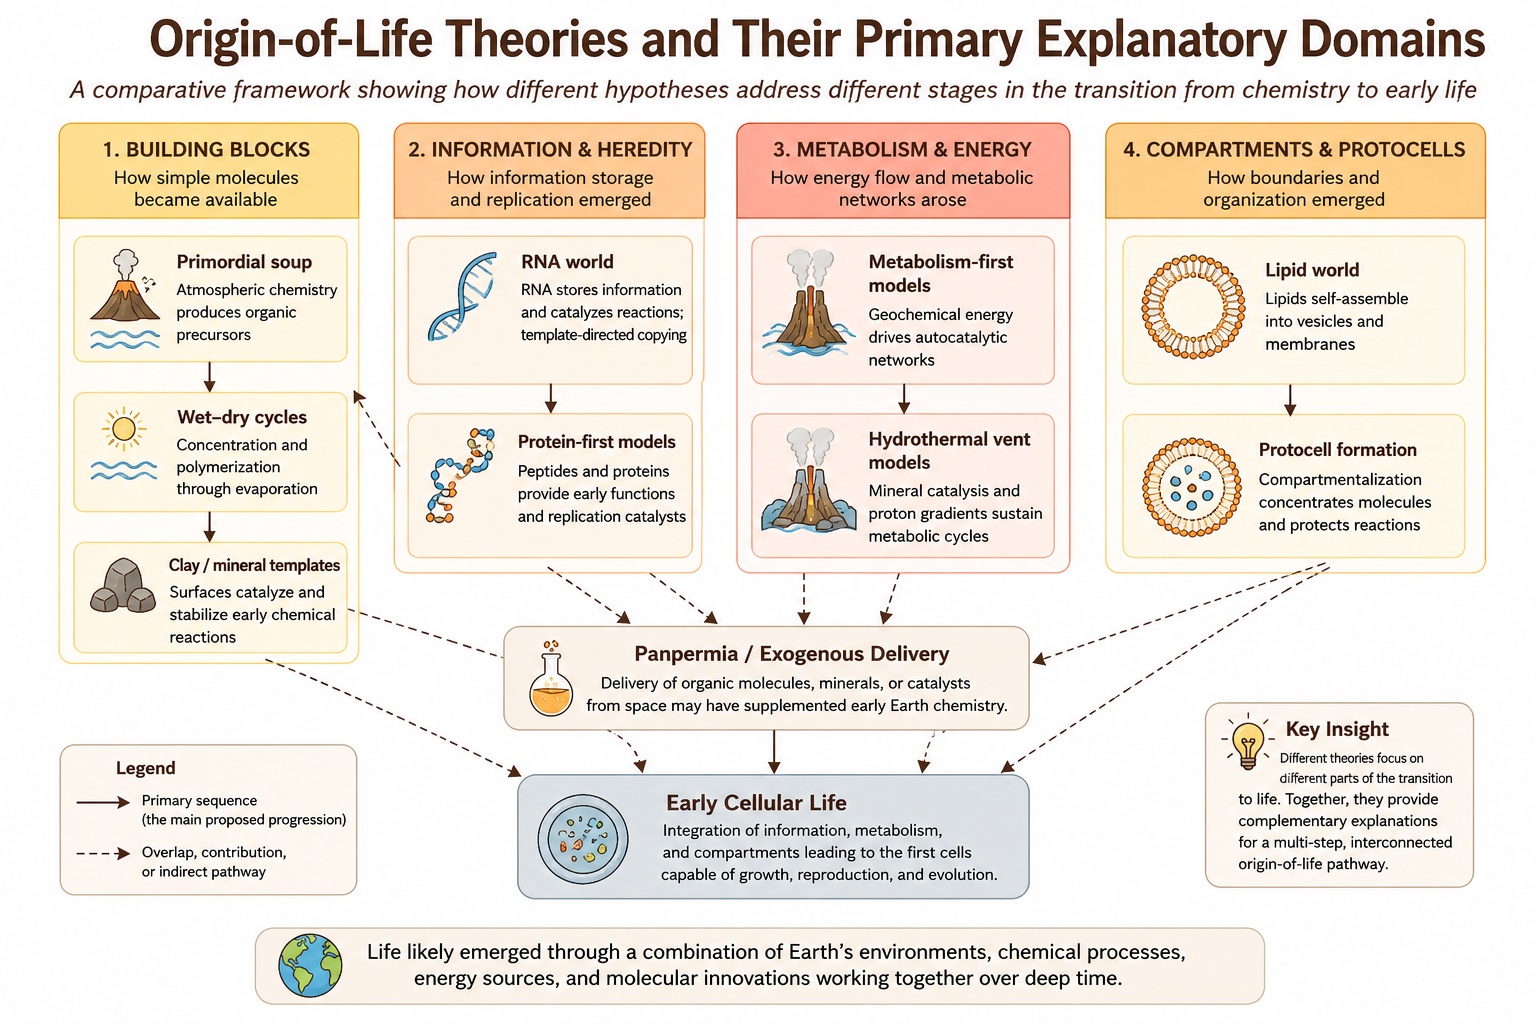
\includegraphics[width=1\linewidth]{figures/01_theory_map} \caption{Conceptual map of major origin-of-life theories and their primary explanatory domains.}\label{fig:theory-map}
\end{figure}

\chapter{Introduction}\label{introduction}

The origin of life remains one of the most profound unresolved questions in modern science. Although evolutionary biology explains how life diversifies through natural selection, the processes that transformed non-living chemistry into the first living systems remain uncertain. Understanding this transition requires contributions from multiple scientific disciplines, including chemistry, molecular biology, geology, planetary science, thermodynamics, and systems theory.

Over the past century, numerous origin-of-life theories have been proposed to explain different stages of this transition. Some models focus on the abiotic synthesis of organic molecules under early Earth conditions, whereas others emphasize the emergence of self-organizing chemical systems, informational polymers such as RNA, primitive metabolic networks, or membrane-bound protocells. Additional hypotheses investigate the catalytic role of mineral surfaces, hydrothermal environments, wet--dry cycling, or the extraterrestrial delivery of organic compounds.

Importantly, these theories do not necessarily compete as mutually exclusive explanations. Instead, many may describe different stages within a broader progression from geochemistry to early biological evolution. This systems perspective forms the central conceptual framework of this book.

\section{The Complexity of Abiogenesis}\label{the-complexity-of-abiogenesis}

Any comprehensive explanation for the origin of life must account for several major scientific transitions. Early Earth chemistry needed to generate organic building blocks, organize them into increasingly complex chemical systems, develop mechanisms for information storage and replication, and ultimately produce populations capable of Darwinian evolution.

Figure \ref{fig:four-hurdles} summarizes four major hurdles that any successful origin-of-life theory must ultimately address.

\begin{figure}
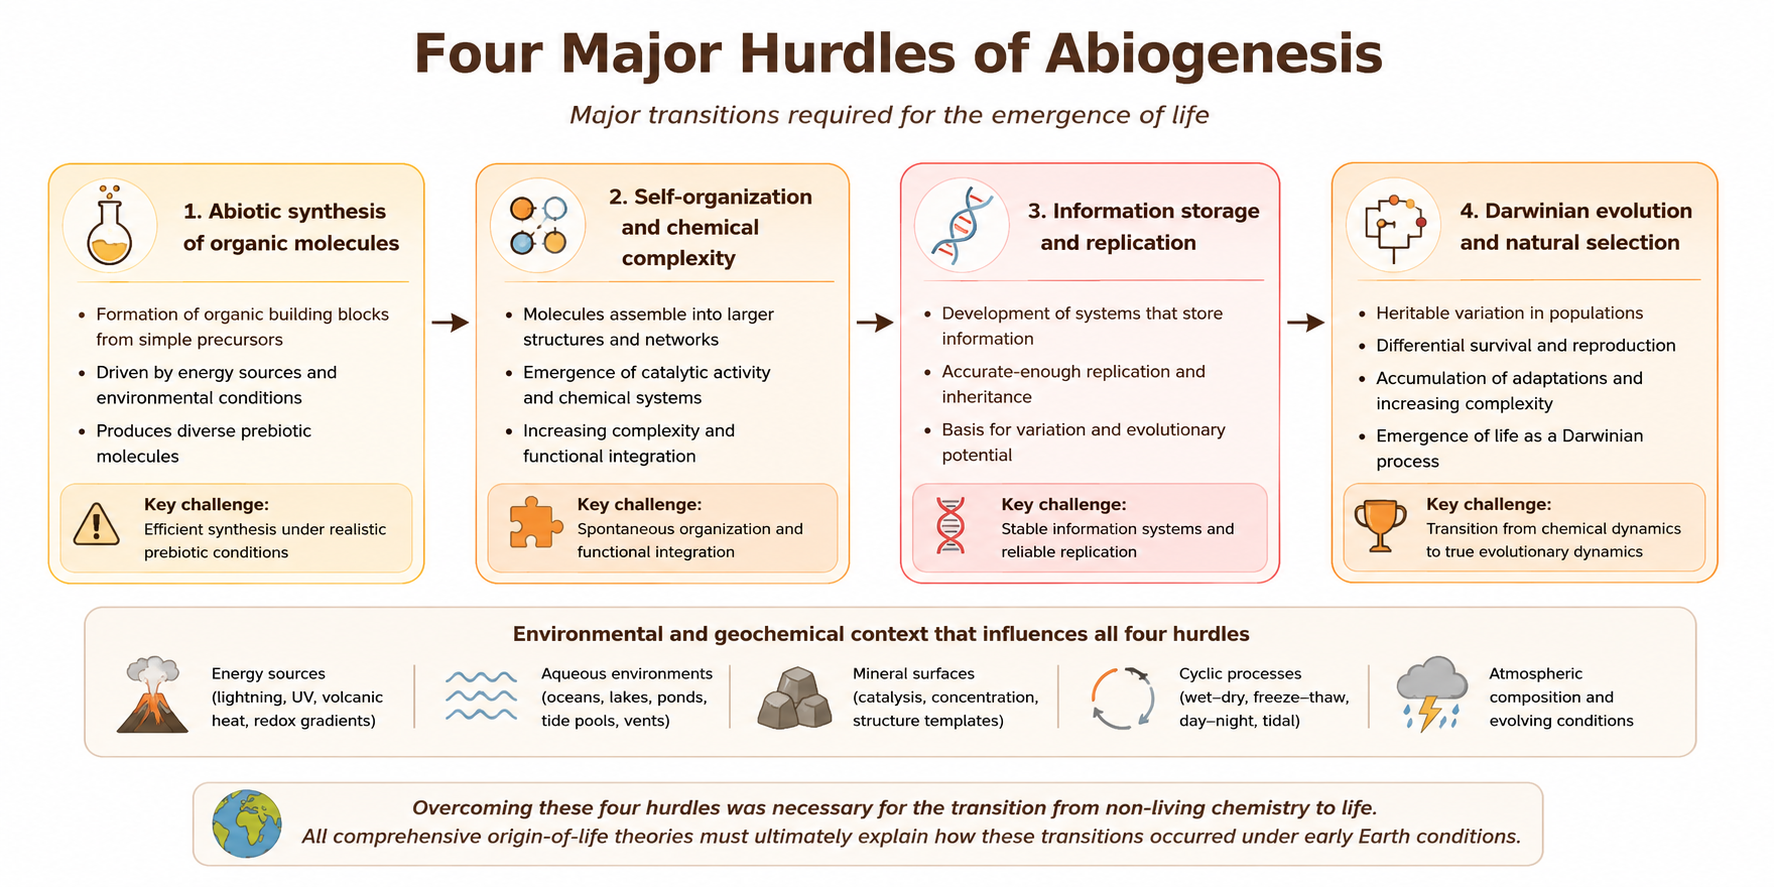
\includegraphics[width=1\linewidth]{figures/02_hurdles_abiogenesis} \caption{Four major hurdles that any comprehensive origin-of-life theory must address.}\label{fig:four-hurdles}
\end{figure}

The first hurdle involves the abiotic synthesis of biologically relevant organic molecules such as amino acids, nucleotides, lipids, and simple sugars. The second concerns the emergence of chemical organization and increasing molecular complexity, including polymer formation and catalytic interactions. The third hurdle requires mechanisms for information storage, replication, and heredity, which are necessary for preserving and transmitting molecular structure across generations. Finally, life requires systems capable of variation, selection, and adaptive evolution.

These challenges are deeply interconnected and remain difficult to explain simultaneously within a single unified framework. As a result, modern origin-of-life research increasingly explores the possibility that multiple mechanisms operated together under early Earth conditions.

\section{Sequential and Hybrid Models of Life's Emergence}\label{sequential-and-hybrid-models-of-lifes-emergence}

Rather than viewing abiogenesis as a single event, many modern researchers interpret it as a gradual sequence of transitions occurring over extended geological timescales. In this view, different origin-of-life theories may explain different stages within a larger pathway from geochemistry to primitive cellular evolution.

Figure \ref{fig:pathway-timeline} illustrates a simplified conceptual progression linking major stages in the transition from non-living chemistry to early biological systems.

\begin{figure}
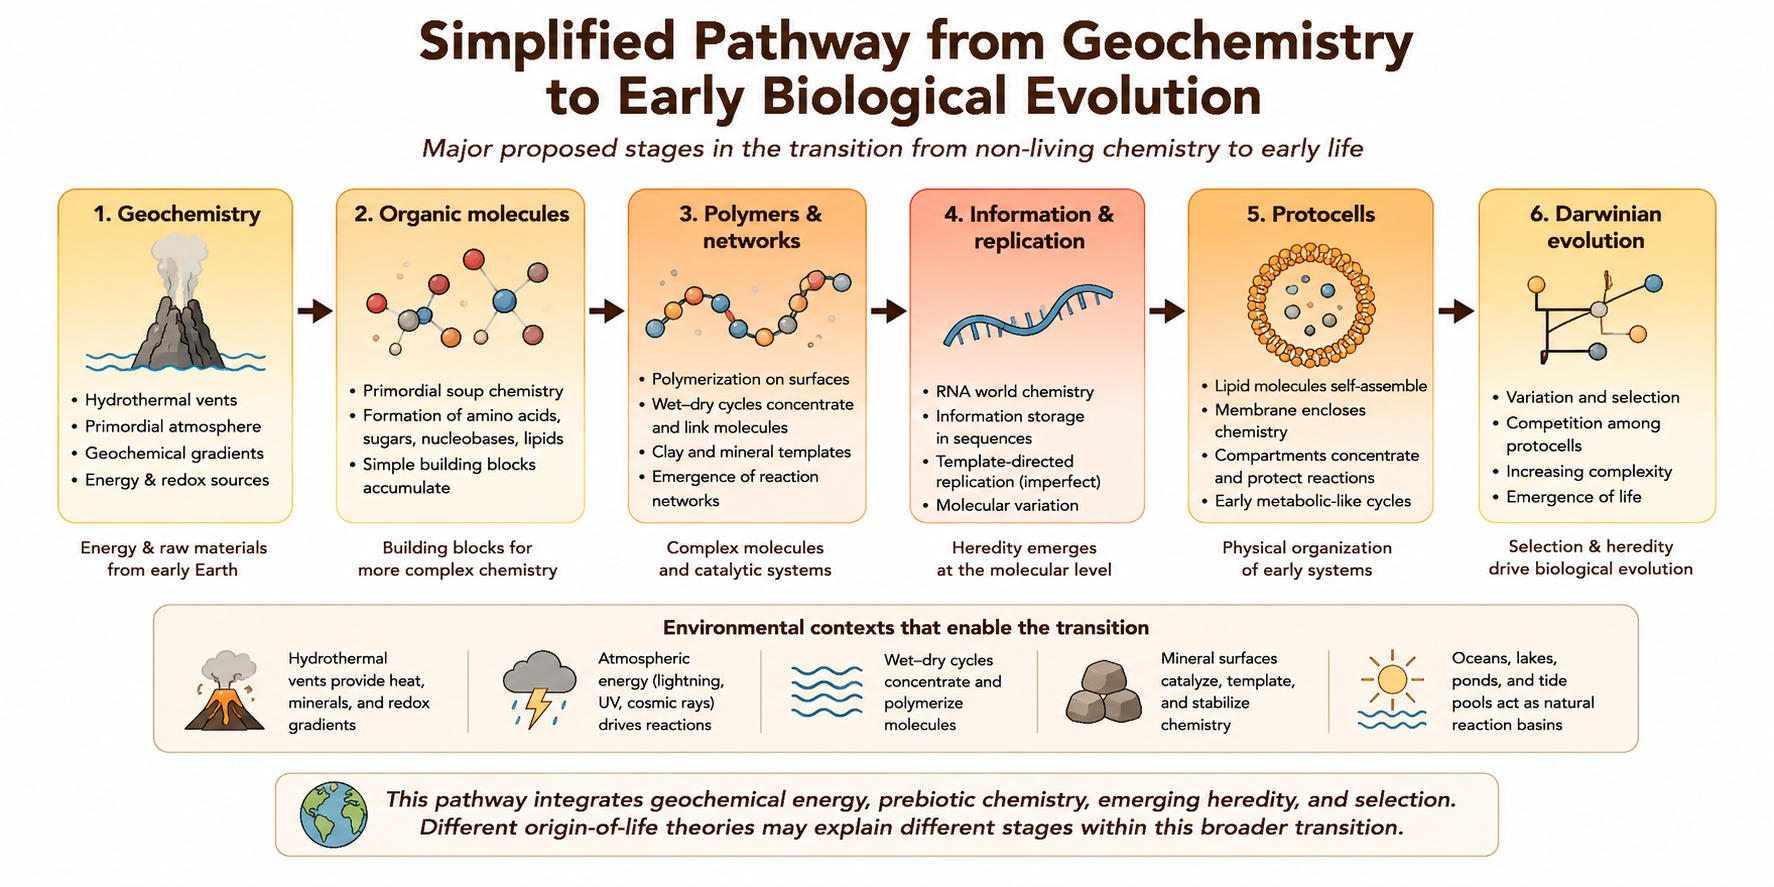
\includegraphics[width=1\linewidth]{figures/03_origin_pathway_timeline} \caption{Simplified pathway showing major proposed stages in the transition from geochemistry to biological evolution and examples of theories associated with each stage.}\label{fig:pathway-timeline}
\end{figure}

In this framework, geochemical environments such as hydrothermal systems or the early atmosphere may have contributed to the synthesis of organic molecules. Wet--dry cycles, mineral surfaces, and related mechanisms may have promoted polymer formation and increasing chemical organization. RNA-based or protein-assisted systems may then have introduced primitive heredity and replication, while lipid membranes and protocell formation may have stabilized increasingly complex chemical networks.

This staged interpretation helps explain why no individual theory fully resolves the origin-of-life problem. Different models may contribute to different transitions within the overall emergence of life.

\section{Methodological Approach}\label{methodological-approach}

This book evaluates each major origin-of-life theory using a consistent comparative framework based on:

\begin{enumerate}
\def\labelenumi{\arabic{enumi}.}
\tightlist
\item
  Explanatory scope
\item
  Mechanistic plausibility
\item
  Experimental and empirical support
\item
  Environmental realism
\item
  Remaining unresolved gaps
\item
  Integrative potential with other models
\end{enumerate}

The goal is not to identify a single ``winning'' theory, but to evaluate which mechanisms appear scientifically plausible, experimentally testable, and potentially compatible within broader hybrid models of abiogenesis.

The chapters that follow examine each major theory individually before comparing their explanatory strengths, limitations, and possible integration into larger systems-level models for the emergence of life.

\chapter{Primordial Soup and Chemical Evolution}\label{primordial-soup-and-chemical-evolution}

\section{Chapter Overview}\label{chapter-overview}

This chapter examines the primordial soup hypothesis as one of the earliest and most influential models of abiotic chemical evolution. The discussion begins with the historical origins of the theory, followed by its mechanistic foundations, environmental setting, experimental evidence, explanatory strengths, major criticisms, and current scientific standing within modern origin-of-life research.

\section{Key Terms}\label{key-terms}

\begin{itemize}
\tightlist
\item
  Abiogenesis
\item
  Prebiotic chemistry
\item
  Chemical evolution
\item
  Reducing atmosphere
\item
  Organic synthesis
\item
  Amino acids
\item
  Nucleobases
\item
  Primordial soup
\end{itemize}

\section{Core Idea}\label{core-idea}

The primordial soup model proposes that the building blocks of life formed through abiotic chemical reactions occurring in early Earth environments. According to this hypothesis, simple inorganic molecules present in the primitive atmosphere, oceans, or shallow water bodies gradually reacted under the influence of external energy sources to produce increasingly complex organic compounds.

Over time, these organic molecules may have accumulated within the early oceans, ponds, or other localized environments, forming a chemically rich ``soup'' from which more advanced prebiotic systems could eventually emerge.

\section{Historical Context}\label{historical-context}

The modern scientific formulation of this idea was independently proposed during the 1920s by Alexander Oparin and J.B.S. Haldane. Both scientists argued that the early Earth atmosphere differed substantially from the modern oxygen-rich atmosphere and may have provided favorable conditions for abiotic organic synthesis.

The hypothesis gained major experimental support in 1953 through the Miller--Urey experiment, in which Stanley Miller demonstrated that amino acids and other organic compounds could form under simulated early Earth conditions involving methane, ammonia, hydrogen, water vapor, and electrical discharge (\citeproc{ref-miller1953}{Miller 1953}).

This experiment became one of the foundational milestones in origin-of-life research because it showed that biologically relevant molecules did not necessarily require living organisms for their formation.

\section{Mechanistic Basis}\label{mechanistic-basis}

To understand why the primordial soup model became influential, it is necessary to examine the chemical mechanisms underlying the theory.

The primordial soup framework proposes that simple atmospheric and geochemical compounds---including water vapor, methane, ammonia, carbon dioxide, hydrogen, and nitrogen-containing molecules---underwent chemical reactions driven by energy sources such as:

\begin{itemize}
\tightlist
\item
  Lightning discharges
\item
  Ultraviolet radiation
\item
  Volcanic heat
\item
  Hydrothermal activity
\item
  Impact-related energy
\end{itemize}

These reactions may have generated amino acids, nucleobases, lipids, sugars, and other biologically relevant organic compounds. Subsequent concentration processes, evaporation cycles, mineral interactions, or localized environmental conditions may then have increased chemical complexity further.

Figure \ref{fig:primordial-soup-pathway-fig} summarizes the simplified chemical progression proposed by the primordial soup model.

\begin{figure}

{\centering 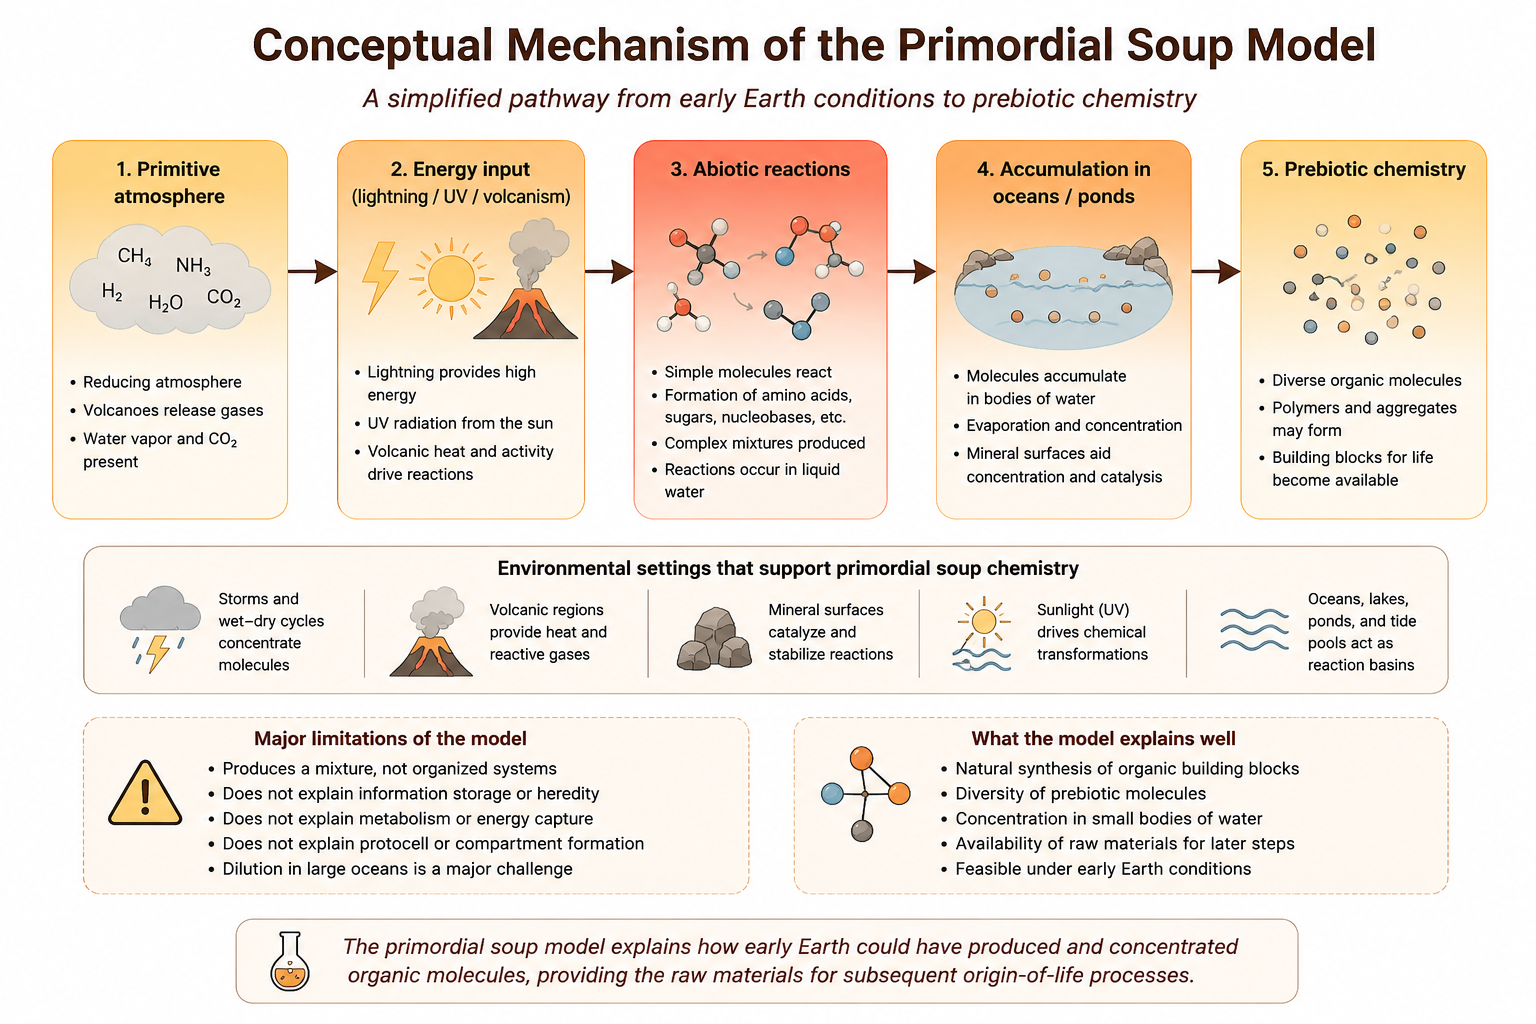
\includegraphics[width=1\linewidth]{figures/04_primordial_soup_pathway} 

}

\caption{Conceptual mechanism of the primordial soup model.}\label{fig:primordial-soup-pathway-fig}
\end{figure}

In many versions of the theory, the accumulation of these molecules created chemically enriched environments capable of supporting additional prebiotic reactions and increasing molecular complexity.

\section{Environmental Setting}\label{environmental-setting}

Early versions of the primordial soup hypothesis often assumed a strongly reducing atmosphere rich in methane, ammonia, hydrogen, and water vapor. Such conditions are chemically favorable for organic synthesis. However, the exact composition of the early Earth atmosphere remains debated, and many modern models suggest it may have been more neutral, containing higher proportions of carbon dioxide, nitrogen, and water vapor.

This uncertainty does not eliminate the possibility of abiotic organic synthesis, but it changes where such synthesis may have been most plausible. Instead of occurring uniformly across the entire atmosphere or ocean, organic production may have been concentrated in localized environments such as volcanic regions, hydrothermal systems, impact sites, shallow ponds, or evaporating pools.

This environmental refinement is important because many prebiotic reactions require not only raw ingredients and energy, but also mechanisms for concentrating molecules and preventing rapid dilution.

\section{What the Theory Explains Well}\label{what-the-theory-explains-well}

The primordial soup model is particularly strong at explaining the abiotic synthesis of prebiotic chemical building blocks. Laboratory experiments and astronomical observations demonstrate that many biologically relevant organic molecules can form naturally under non-biological conditions.

The theory also provides a chemically intuitive starting point for abiogenesis by showing that complex organic chemistry can emerge from relatively simple inorganic precursors under plausible environmental conditions.

The significance of the primordial soup hypothesis extends beyond the origin of life itself. It helped establish the idea that the boundary between chemistry and biology may be gradual rather than abrupt.

\section{What Makes It Plausible}\label{what-makes-it-plausible}

Several lines of evidence support the plausibility of primordial soup chemistry:

\begin{itemize}
\tightlist
\item
  Laboratory synthesis experiments can generate organic compounds under simulated prebiotic conditions
\item
  Carbonaceous meteorites contain amino acids and diverse organic molecules
\item
  Organic chemistry occurs naturally in interstellar clouds, comets, and planetary environments
\item
  Volcanic, hydrothermal, and impact environments provide realistic energy gradients capable of driving chemical reactions
\item
  Wet--dry or evaporative settings may help concentrate organic compounds
\end{itemize}

Together, these observations support the idea that abiotic organic synthesis is chemically feasible on planetary bodies.

\section{Key Experimental and Observational Support}\label{key-experimental-and-observational-support}

The Miller--Urey experiment remains the most iconic demonstration of abiotic organic synthesis (\citeproc{ref-miller1953}{Miller 1953}). Later experiments using revised atmospheric compositions and alternative energy sources have also generated amino acids, nucleobases, and lipid precursors under a variety of simulated early Earth conditions.

In addition, analyses of carbonaceous chondrite meteorites such as the Murchison meteorite have revealed numerous organic compounds, including amino acids and nitrogen-containing molecules. These findings suggest that prebiotic organic chemistry may occur naturally both on Earth and in extraterrestrial environments.

This evidence does not prove that life began in a global oceanic soup, but it strongly supports the broader claim that organic precursor molecules can form through natural chemical processes.

\section{Major Gaps and Critiques}\label{major-gaps-and-critiques}

Despite its strengths, the primordial soup model faces several major limitations.

Most importantly, the theory explains the production of chemical ingredients but does not adequately explain how these molecules became organized into self-sustaining, information-bearing systems capable of replication and evolution.

Additional challenges include:

\begin{itemize}
\tightlist
\item
  Dilution of organic molecules in large ocean environments
\item
  Instability of some biomolecules in aqueous conditions
\item
  Difficulty forming long polymers spontaneously
\item
  Lack of a clear mechanism for heredity or metabolic organization
\item
  Uncertainty regarding the exact composition of the early Earth atmosphere
\item
  Limited explanation for compartment formation and protocell development
\end{itemize}

For these reasons, primordial soup models are generally considered necessary but insufficient explanations for the complete emergence of life.

\section{Integration with Other Theories}\label{integration-with-other-theories}

The primordial soup model is most powerful when viewed as one component of a broader origin-of-life framework. It may explain the source of organic building blocks that later participated in other prebiotic processes.

For example, organic compounds produced through atmospheric chemistry, hydrothermal reactions, or extraterrestrial delivery could have been concentrated by wet--dry cycles, organized on mineral surfaces, incorporated into lipid compartments, or used in early RNA-like systems.

In this sense, primordial soup chemistry may provide the ingredients, while other theories attempt to explain organization, replication, metabolism, and compartmentalization.

\section{Systems Perspective}\label{systems-perspective}

The primordial soup model primarily addresses the first major hurdle of abiogenesis: the synthesis of organic building blocks. However, the theory alone does not fully explain how these molecules became organized into replicating and evolving systems.

Consequently, modern origin-of-life research often combines primordial synthesis models with theories involving mineral catalysis, self-organization, RNA heredity, metabolism-first pathways, or protocell formation.

This makes the primordial soup hypothesis foundational, but not complete.

\section{Modern Relevance}\label{modern-relevance}

The primordial soup framework also remains important in modern astrobiology. Because abiotic organic synthesis appears chemically feasible under a range of planetary conditions, similar processes may occur on Mars, icy moons, comets, meteorites, or exoplanets with suitable chemical ingredients and energy sources.

The theory therefore contributes not only to understanding life's origin on Earth, but also to broader questions about where life might emerge elsewhere in the universe.

\section{Current Scientific Standing}\label{current-scientific-standing}

The primordial soup framework remains one of the foundational models in origin-of-life research and continues to play a central role in prebiotic chemistry. Most modern researchers accept that abiotic organic synthesis likely occurred on the early Earth to some extent.

However, contemporary origin-of-life studies increasingly view primordial soup chemistry as one component within a larger sequence of prebiotic transitions rather than a complete standalone explanation for abiogenesis. Modern hybrid models often integrate primordial synthesis with mineral catalysis, hydrothermal environments, RNA-based heredity, metabolism-first chemistry, or protocell formation.

\section{Comparative Assessment}\label{comparative-assessment}

\begin{longtable}[]{@{}
  >{\raggedright\arraybackslash}p{(\columnwidth - 2\tabcolsep) * \real{0.5000}}
  >{\raggedright\arraybackslash}p{(\columnwidth - 2\tabcolsep) * \real{0.5000}}@{}}
\toprule\noalign{}
\begin{minipage}[b]{\linewidth}\raggedright
Dimension
\end{minipage} & \begin{minipage}[b]{\linewidth}\raggedright
Assessment
\end{minipage} \\
\midrule\noalign{}
\endhead
\bottomrule\noalign{}
\endlastfoot
Primary Contribution & Abiotic synthesis of organic building blocks \\
Explanatory Strength & Strong for precursor chemistry \\
Mechanistic Plausibility & High \\
Experimental Support & Strong for organic synthesis \\
Environmental Realism & Plausible, but dependent on local conditions \\
Main Limitation & Does not explain organization, heredity, or evolution \\
Integrative Potential & High \\
Current Scientific Standing & Foundational but incomplete component of abiogenesis models \\
\end{longtable}

\section{Comparative Performance}\label{comparative-performance}

\begin{longtable}[]{@{}ll@{}}
\toprule\noalign{}
Question & Primordial Soup Performance \\
\midrule\noalign{}
\endhead
\bottomrule\noalign{}
\endlastfoot
Produces organic building blocks? & Strong \\
Explains polymer formation? & Limited \\
Explains heredity? & Weak \\
Explains metabolism? & Limited \\
Explains compartment formation? & Weak \\
Supported experimentally? & Strong \\
Useful in hybrid models? & Strong \\
\end{longtable}

\chapter{RNA World Hypothesis}\label{rna-world-hypothesis}

\section{Chapter Overview}\label{chapter-overview-1}

This chapter examines the RNA World hypothesis, one of the most influential models in origin-of-life research. The chapter explains why RNA is considered a possible bridge between chemistry and biology, reviews its historical development, describes its proposed mechanism, evaluates supporting evidence, and discusses the major challenges that remain.

\section{Key Terms}\label{key-terms-1}

\begin{itemize}
\tightlist
\item
  RNA World
\item
  Ribozyme
\item
  Heredity
\item
  Catalysis
\item
  Replication
\item
  Molecular evolution
\item
  Information storage
\item
  Proto-selection
\end{itemize}

\section{Core Idea}\label{core-idea-1}

The RNA World hypothesis proposes that RNA preceded DNA and proteins as the central molecule of early biological systems. The hypothesis is powerful because RNA can perform two functions that are essential for life: it can store genetic information and, in some cases, catalyze chemical reactions (\citeproc{ref-gilbert1986}{Gilbert 1986}).

In modern life, DNA primarily stores genetic information, proteins perform most catalytic functions, and RNA acts as an intermediary between them. The RNA World hypothesis suggests that, before this division of labour evolved, RNA may have carried out both informational and catalytic roles.

\section{Historical Context}\label{historical-context-1}

The term ``RNA World'' was formalized by Walter Gilbert in 1986 (\citeproc{ref-gilbert1986}{Gilbert 1986}), but the idea developed from earlier discoveries in molecular biology. The discovery of catalytic RNA molecules, known as ribozymes, showed that RNA was not merely a passive messenger molecule but could also participate directly in chemical catalysis.

This discovery was significant because it provided a possible solution to a major origin-of-life problem: which came first, genetic information or functional enzymes? If RNA could perform both roles, then early life may not have required separate DNA genomes and protein enzymes at the beginning.

\section{Mechanistic Basis}\label{mechanistic-basis-1}

The RNA World hypothesis proposes that early RNA-like molecules formed, copied themselves imperfectly, and underwent selection based on their stability, catalytic ability, and replication efficiency. In this framework, RNA acted as a bridge between prebiotic chemistry and biological evolution.

RNA is proposed to have supported early life-like systems through four related functions:

\begin{itemize}
\tightlist
\item
  Storing sequence-based information
\item
  Catalyzing chemical reactions
\item
  Supporting copying or template-directed replication
\item
  Allowing variation and selection among molecular populations
\end{itemize}

Figure \ref{fig:rna-world-mechanism-fig} summarizes the mechanistic logic of the RNA World hypothesis.

\begin{figure}

{\centering 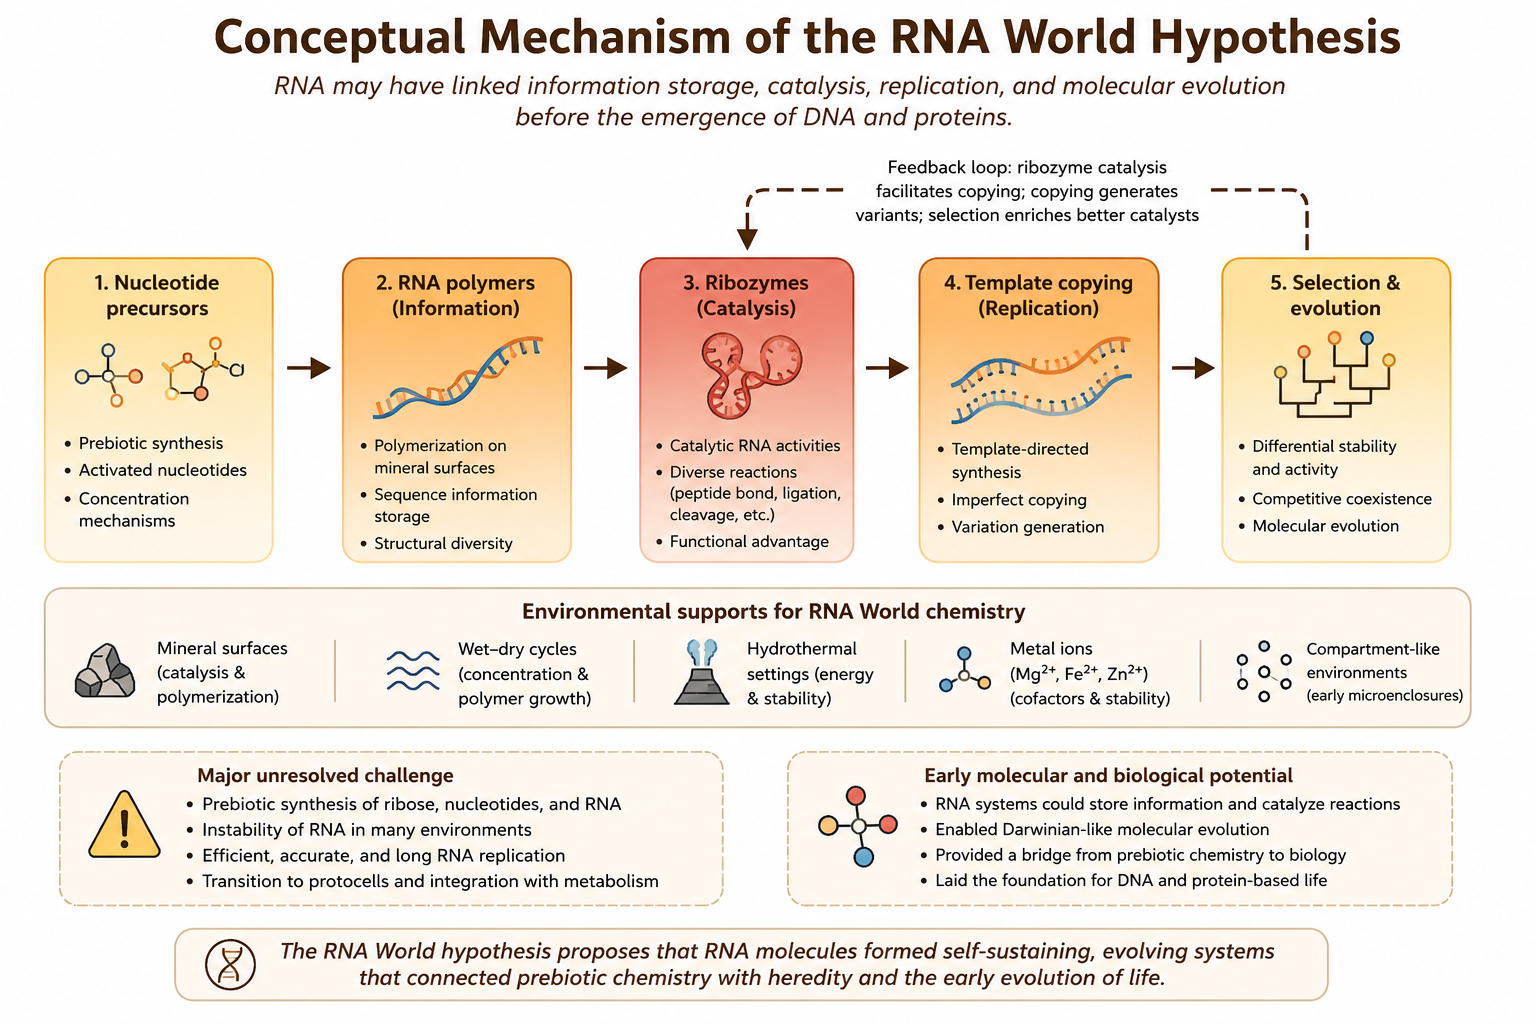
\includegraphics[width=1\linewidth]{figures/04_rna_world_mechanism} 

}

\caption{Conceptual mechanism of the RNA World hypothesis.}\label{fig:rna-world-mechanism-fig}
\end{figure}

The figure illustrates why RNA remains central to origin-of-life research: it provides a plausible molecular link between chemical complexity and Darwinian evolution.

\section{What the Theory Explains Well}\label{what-the-theory-explains-well-1}

The RNA World hypothesis is strongest at explaining the emergence of heredity and pre-cellular molecular evolution. Unlike the primordial soup model, which mainly explains the formation of organic ingredients, the RNA World hypothesis directly addresses how information could be stored, copied, and modified over time.

This makes the theory especially important because heredity is one of the defining features of life. Without some mechanism for information transfer, chemical systems may become complex, but they cannot evolve in a Darwinian sense.

\section{What Makes It Plausible}\label{what-makes-it-plausible-1}

Several features make the RNA World hypothesis scientifically plausible.

First, RNA can store information in its nucleotide sequence. Second, some RNA molecules can act as ribozymes and catalyze reactions. Third, RNA plays central roles in modern cells, including in translation, gene regulation, and protein synthesis. The ribosome itself contains a catalytic RNA core, suggesting that RNA may preserve traces of an ancient biochemical world (\citeproc{ref-joyce2002}{Joyce 2002}).

These observations suggest that RNA is not simply a later accessory molecule, but may have played a deeper role in the early evolution of biological systems.

\section{Key Experimental and Observational Support}\label{key-experimental-and-observational-support-1}

The strongest support for the RNA World hypothesis comes from the discovery and study of catalytic ribozymes. Ribozymes demonstrate that RNA can catalyze reactions without proteins, supporting the idea that early biological systems may have relied on RNA-based catalysis.

In vitro evolution experiments also show that RNA molecules can be selected for specific catalytic or binding functions under laboratory conditions (\citeproc{ref-joyce2002}{Joyce 2002}). These experiments demonstrate that RNA populations can undergo variation and selection, which are essential ingredients for molecular evolution.

Additional support comes from the central role of RNA in modern biology. Ribosomal RNA performs the key catalytic step in protein synthesis, and many essential cellular processes still depend on RNA-based mechanisms.

\section{Major Gaps and Critiques}\label{major-gaps-and-critiques-1}

Despite its strengths, the RNA World hypothesis faces major challenges.

The most important gap is prebiotic accessibility. RNA is chemically complex, relatively fragile, and difficult to synthesize under realistic early Earth conditions. Forming ribose sugars, nucleobases, phosphate groups, and linking them into stable nucleotides remains a major chemical problem.

Additional challenges include:

\begin{itemize}
\tightlist
\item
  Difficulty producing RNA nucleotides under plausible prebiotic conditions
\item
  Instability of RNA in many environmental settings
\item
  The challenge of forming long RNA polymers
\item
  The difficulty of achieving accurate RNA replication without enzymes
\item
  The need for concentration mechanisms to prevent dilution
\item
  The lack of clear explanation for how RNA systems became enclosed in protocells
\end{itemize}

For these reasons, many researchers consider the RNA World hypothesis powerful but incomplete.

\section{Integration with Other Theories}\label{integration-with-other-theories-1}

The RNA World hypothesis is often treated as part of a broader hybrid model of abiogenesis. It may explain the emergence of heredity, but it likely required support from other prebiotic processes.

For example, primordial soup chemistry may have supplied some organic precursors. Wet--dry cycles or mineral surfaces may have helped concentrate and polymerize nucleotides. Lipid compartments may have protected RNA molecules and allowed early protocells to form. Metabolic or geochemical systems may also have supplied energy and chemical scaffolding.

In this broader view, the RNA World may not represent the very beginning of abiogenesis, but rather an important intermediate stage between prebiotic chemistry and early cellular life.

\section{Systems Perspective}\label{systems-perspective-1}

Within the comparative framework of this book, the RNA World hypothesis primarily addresses the third major hurdle of abiogenesis: information storage and replication.

Its greatest contribution is that it offers a plausible route from chemistry to heredity. However, it does not fully explain the earlier formation of RNA building blocks, nor does it independently explain metabolism or compartment formation.

Therefore, the RNA World hypothesis is best understood as a central but partial explanation within a larger systems-level model of life's emergence.

\section{Modern Relevance}\label{modern-relevance-1}

The RNA World hypothesis continues to influence modern origin-of-life research, synthetic biology, molecular evolution, and astrobiology. It provides a model for how simple molecular systems might begin to evolve before the appearance of DNA genomes and protein enzymes.

The hypothesis also helps explain why RNA remains so deeply embedded in modern biology. Its central role in translation, regulation, and catalysis may reflect an ancient evolutionary legacy.

\section{Current Scientific Standing}\label{current-scientific-standing-1}

The RNA World hypothesis remains one of the most influential origin-of-life theories. It is widely regarded as a strong explanation for the emergence of heredity and early molecular evolution.

However, most current interpretations do not treat RNA World as a complete standalone theory. Instead, RNA-based systems are often viewed as one phase within a broader sequence involving prebiotic chemistry, environmental concentration, mineral catalysis, energy flow, and protocell formation.

\section{Comparative Assessment}\label{comparative-assessment-1}

\begin{longtable}[]{@{}
  >{\raggedright\arraybackslash}p{(\columnwidth - 2\tabcolsep) * \real{0.5000}}
  >{\raggedright\arraybackslash}p{(\columnwidth - 2\tabcolsep) * \real{0.5000}}@{}}
\toprule\noalign{}
\begin{minipage}[b]{\linewidth}\raggedright
Dimension
\end{minipage} & \begin{minipage}[b]{\linewidth}\raggedright
Assessment
\end{minipage} \\
\midrule\noalign{}
\endhead
\bottomrule\noalign{}
\endlastfoot
Primary Contribution & Information storage, catalysis, and early heredity \\
Explanatory Strength & Strong for heredity and molecular evolution \\
Mechanistic Plausibility & Moderate to high \\
Experimental Support & Strong for ribozymes and RNA evolution \\
Environmental Realism & Challenging due to RNA synthesis and instability \\
Main Limitation & Difficulty forming and replicating RNA under prebiotic conditions \\
Integrative Potential & High \\
Current Scientific Standing & Central but incomplete component of abiogenesis models \\
\end{longtable}

\section{Comparative Performance}\label{comparative-performance-1}

\begin{longtable}[]{@{}
  >{\raggedright\arraybackslash}p{(\columnwidth - 2\tabcolsep) * \real{0.5000}}
  >{\raggedright\arraybackslash}p{(\columnwidth - 2\tabcolsep) * \real{0.5000}}@{}}
\toprule\noalign{}
\begin{minipage}[b]{\linewidth}\raggedright
Question
\end{minipage} & \begin{minipage}[b]{\linewidth}\raggedright
RNA World Performance
\end{minipage} \\
\midrule\noalign{}
\endhead
\bottomrule\noalign{}
\endlastfoot
Produces organic building blocks? & Weak to limited \\
Explains polymer formation? & Moderate, but chemically challenging \\
Explains heredity? & Strong \\
Explains catalysis? & Strong \\
Explains metabolism? & Limited \\
Explains compartment formation? & Weak \\
Supported experimentally? & Strong for ribozymes and in vitro evolution \\
Useful in hybrid models? & Strong \\
\end{longtable}

\chapter{Metabolism-First and Hydrothermal Vent Theories}\label{metabolism-first-and-hydrothermal-vent-theories}

\section{Chapter Overview}\label{chapter-overview-2}

This chapter examines metabolism-first and hydrothermal vent theories, which propose that organized energy-driven chemical networks may have emerged before modern genetic systems. Unlike RNA-centered models that prioritize heredity, these theories emphasize geochemistry, catalytic surfaces, energy gradients, and self-sustaining metabolic reactions as the earliest foundations of life.

The chapter reviews the historical development of metabolism-first models, their mechanistic foundations, supporting evidence, major criticisms, and their role within modern hybrid models of abiogenesis.

\section{Key Terms}\label{key-terms-2}

\begin{itemize}
\tightlist
\item
  Metabolism-first
\item
  Hydrothermal vents
\item
  Proton gradients
\item
  Geochemical energy
\item
  Catalytic surfaces
\item
  Redox chemistry
\item
  Autocatalytic networks
\item
  Alkaline vents
\end{itemize}

\section{Core Idea}\label{core-idea-2}

Metabolism-first theories propose that life began through the emergence of self-organizing chemical reaction networks powered by naturally occurring energy gradients. In this framework, primitive metabolic processes may have developed before fully formed genetic systems such as RNA or DNA.

Many versions of the theory focus on hydrothermal vent environments, where hot mineral-rich fluids interact with colder ocean water to produce strong chemical disequilibria and continuous energy flow. These environments may have provided natural settings capable of supporting increasingly complex prebiotic chemistry (\citeproc{ref-martin2008}{Martin et al. 2008}; \citeproc{ref-wachtershauser1988}{Wächtershäuser 1988}).

Rather than beginning with heredity, metabolism-first models propose that the earliest steps toward life involved energy transformation, catalytic chemistry, and geochemically sustained reaction systems.

\section{Historical Context}\label{historical-context-2}

Metabolism-first ideas emerged partly in response to limitations in earlier origin-of-life models. Although primordial soup and RNA World theories explain important aspects of prebiotic chemistry and heredity, they do not fully explain how early systems obtained continuous energy or maintained organized chemical activity.

One influential metabolism-first framework was proposed by Günter Wächtershäuser, who suggested that life may have originated on mineral surfaces rich in iron and sulfur compounds (\citeproc{ref-wachtershauser1988}{Wächtershäuser 1988}). Later work by Michael Russell, William Martin, and others emphasized alkaline hydrothermal vent systems as plausible environments for early metabolic organization (\citeproc{ref-martin2008}{Martin et al. 2008}).

These theories shifted attention from isolated molecules toward dynamic geochemical systems capable of sustaining continuous chemical reactions.

\section{Mechanistic Basis}\label{mechanistic-basis-2}

To understand metabolism-first theories, it is necessary to examine the role of energy gradients in prebiotic chemistry.

Hydrothermal vent environments naturally generate differences in temperature, pH, redox state, and chemical composition. These gradients can drive reactions that would otherwise be energetically unfavorable. Mineral surfaces containing iron, sulfur, nickel, and related compounds may also act as catalysts that promote organic synthesis and electron transfer reactions.

In metabolism-first models, early chemical systems may have developed through:

\begin{itemize}
\tightlist
\item
  Continuous geochemical energy flow
\item
  Catalytic mineral surfaces
\item
  Redox reactions
\item
  Carbon fixation pathways
\item
  Self-reinforcing chemical cycles
\item
  Proton gradients across mineral compartments
\end{itemize}

Figure \ref{fig:metabolism-first-overview} provides a systems-level overview of the conceptual mechanism proposed by metabolism-first and hydrothermal vent theories.

\begin{figure}
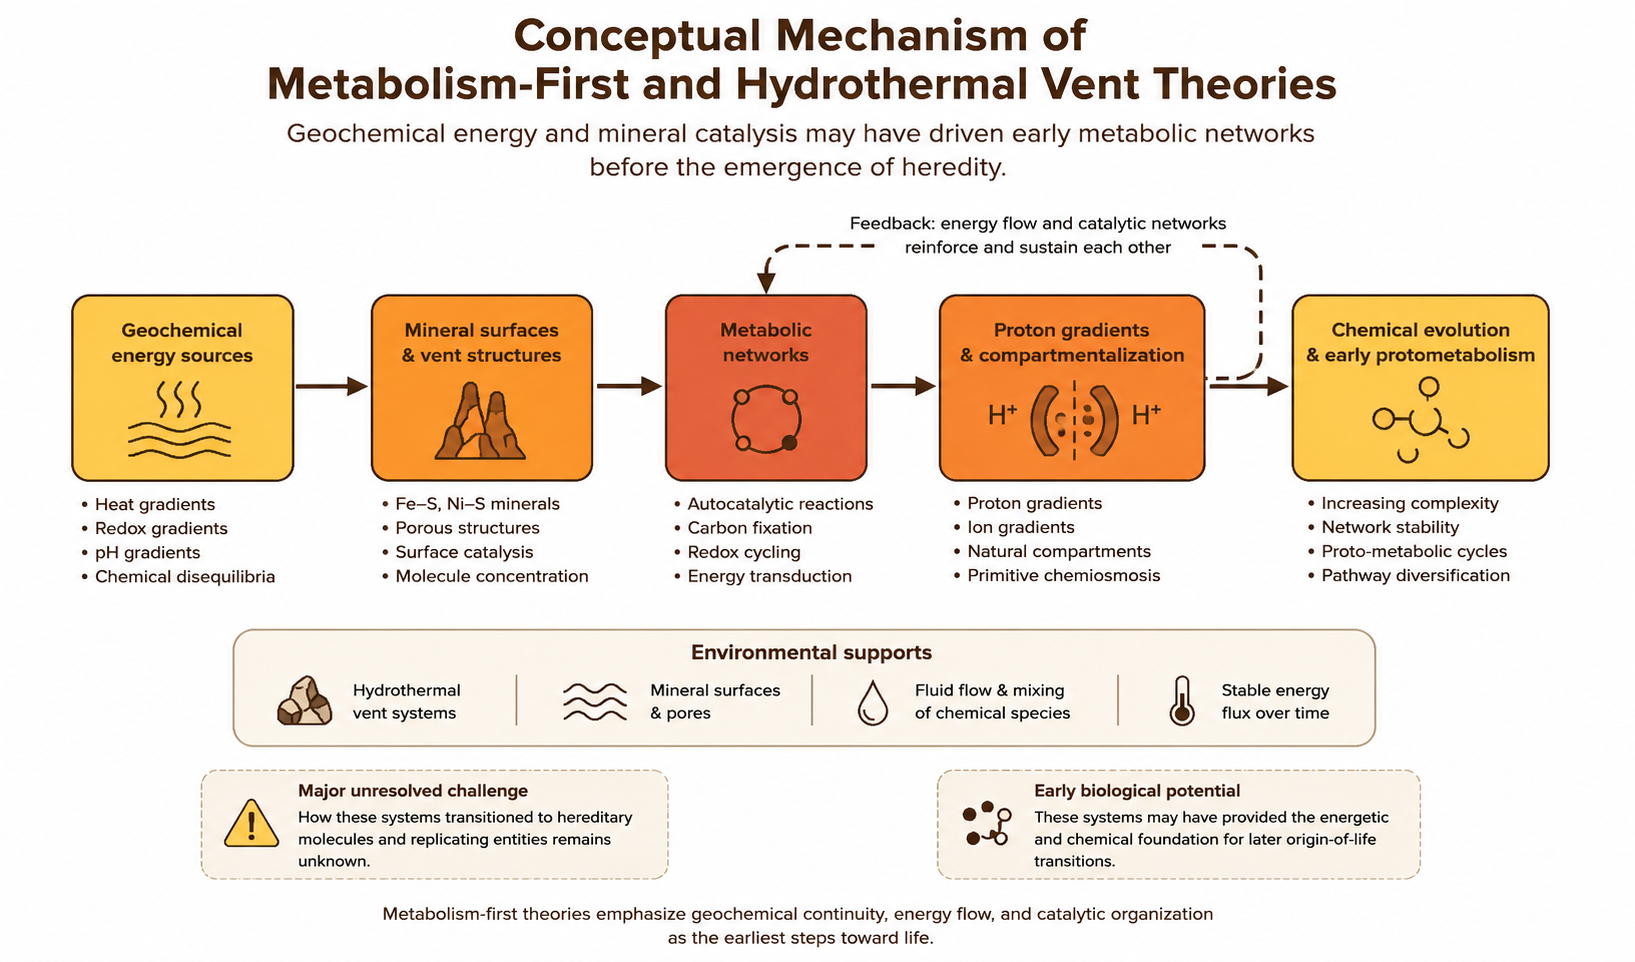
\includegraphics[width=1\linewidth]{figures/05_metabolism_first} \caption{Conceptual mechanism of metabolism-first and hydrothermal vent theories.}\label{fig:metabolism-first-overview}
\end{figure}

The figure illustrates the central idea behind metabolism-first models: naturally occurring geochemical energy gradients and mineral-catalyzed reaction networks may have generated increasingly organized chemical systems before the emergence of heredity.

Unlike RNA-centered hypotheses, these theories prioritize energy flow, catalytic organization, and thermodynamic disequilibrium as the earliest foundations of life.

\section{Hydrothermal Vent Environment}\label{hydrothermal-vent-environment}

Many metabolism-first models focus specifically on alkaline hydrothermal vent systems as plausible environments for prebiotic chemistry.

Hydrothermal vents contain strong gradients in temperature, pH, electron availability, and chemical composition. Mineral-rich vent walls also provide naturally porous structures capable of concentrating molecules and supporting catalytic reactions.

Figure \ref{fig:hydrothermal-vent-schematic} illustrates how hydrothermal vent systems may have generated favorable conditions for early metabolic chemistry.

\begin{figure}
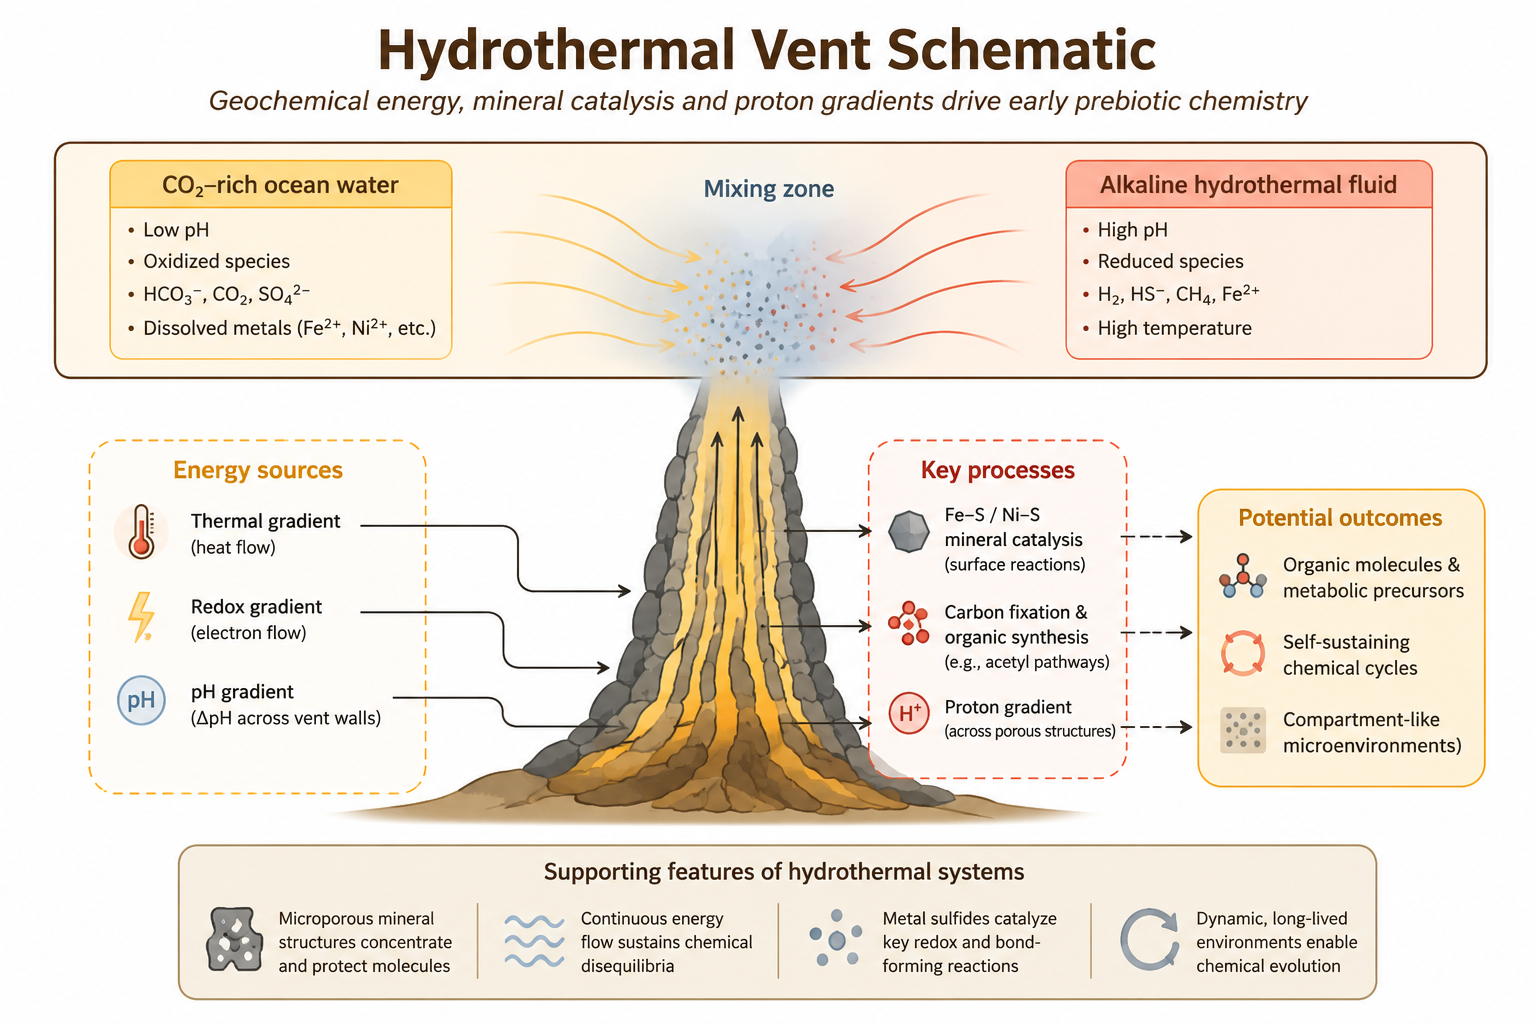
\includegraphics[width=1\linewidth]{figures/05_hydrothermal_vent_schematic} \caption{Hydrothermal vent schematic illustrating geochemical gradients, catalytic surfaces, and potential pathways for prebiotic chemistry.}\label{fig:hydrothermal-vent-schematic}
\end{figure}

The schematic highlights several important features emphasized by hydrothermal vent theories:

\begin{itemize}
\tightlist
\item
  Continuous thermal and chemical energy flow
\item
  Redox disequilibrium between vent fluids and ocean water
\item
  Proton gradients across porous mineral structures
\item
  Iron--sulfur mineral catalysis
\item
  Natural compartment-like microenvironments
\item
  Concentration and stabilization of reacting molecules
\end{itemize}

Together, these features may have allowed early chemical systems to maintain organized reaction networks over extended periods of time.

\section{Environmental Setting}\label{environmental-setting-1}

Hydrothermal vent systems are considered particularly important because they provide long-lasting and chemically active environments capable of sustaining continuous reactions.

Alkaline hydrothermal vents contain naturally occurring microporous mineral structures that resemble primitive compartments. These mineral pores may have concentrated molecules, stabilized reactions, and maintained proton gradients analogous to those used by modern cells for energy production.

Unlike shallow surface environments that experience rapid fluctuations, hydrothermal systems may provide relatively stable conditions over long geological timescales.

This environmental continuity is one of the major strengths of metabolism-first models.

\section{What the Theory Explains Well}\label{what-the-theory-explains-well-2}

Metabolism-first theories are particularly strong at explaining:

\begin{itemize}
\tightlist
\item
  Continuous energy flow
\item
  Geochemical organization
\item
  Catalytic reaction networks
\item
  Carbon fixation pathways
\item
  Environmental continuity between geology and biology
\item
  Natural proton gradients resembling modern bioenergetics
\end{itemize}

These theories provide one of the strongest explanations for how early chemical systems may have maintained organized activity before the appearance of complex hereditary molecules.

The framework is especially important because all living systems require continuous energy processing. Metabolism-first theories therefore address one of the central thermodynamic challenges of abiogenesis.

\section{What Makes It Plausible}\label{what-makes-it-plausible-2}

Several observations support the plausibility of metabolism-first and hydrothermal vent models:

\begin{itemize}
\tightlist
\item
  Modern hydrothermal vents contain rich chemical and thermal gradients
\item
  Many ancient enzymes rely on iron--sulfur clusters similar to vent minerals
\item
  Modern cells universally depend on proton gradients for energy production
\item
  Mineral surfaces can catalyze important organic reactions
\item
  Hydrothermal systems provide natural compartment-like structures
\end{itemize}

These observations suggest that modern biochemistry may preserve traces of ancient geochemical processes.

\section{Key Experimental and Observational Support}\label{key-experimental-and-observational-support-2}

Laboratory experiments demonstrate that mineral surfaces can catalyze organic reactions and support carbon fixation-like pathways under hydrothermal conditions.

Experimental studies have also shown that proton gradients can emerge naturally across mineral barriers, supporting the plausibility of primitive energy transduction systems (\citeproc{ref-martin2008}{Martin et al. 2008}).

Geological evidence further confirms that hydrothermal systems existed on the early Earth and likely represented long-lived chemically active environments.

Although no experiment has fully recreated an origin-of-life pathway, modern research increasingly supports the importance of geochemical energy gradients in prebiotic chemistry.

\section{Major Gaps and Critiques}\label{major-gaps-and-critiques-2}

Despite their strengths, metabolism-first theories face several major limitations.

Most importantly, these models do not fully explain how hereditary systems emerged. Organized metabolism alone is insufficient for Darwinian evolution unless information can also be stored, copied, and transmitted.

Additional challenges include:

\begin{itemize}
\tightlist
\item
  Limited explanation for the origin of genetic information
\item
  Difficulty transitioning from mineral-bound chemistry to free-living cells
\item
  Uncertainty regarding how metabolic cycles became self-sustaining
\item
  Lack of direct evidence for specific early metabolic pathways
\item
  Difficulty reproducing complete metabolic systems experimentally
\end{itemize}

For these reasons, metabolism-first theories are generally viewed as important but incomplete explanations for abiogenesis.

\section{Integration with Other Theories}\label{integration-with-other-theories-2}

Metabolism-first theories integrate naturally with several other origin-of-life models.

Geochemical systems may have produced organic molecules later incorporated into RNA-based heredity systems. Mineral compartments may also have supported protocell development and lipid membrane formation. Wet--dry cycles and primordial synthesis models may have supplied additional chemical precursors.

In many modern hybrid frameworks, metabolism-first chemistry provides the energetic and geochemical foundation upon which heredity and cellular organization later developed.

\section{Systems Perspective}\label{systems-perspective-2}

Within the comparative framework of this book, metabolism-first theories primarily address the second major hurdle of abiogenesis: the emergence of organized chemical systems powered by continuous energy flow.

Their greatest strength lies in explaining how chemistry may have become thermodynamically organized before the appearance of sophisticated biological machinery. However, these theories do not independently explain heredity or fully developed evolutionary systems.

Consequently, metabolism-first models are best understood as one component within broader systems-level explanations of life's emergence.

\section{Modern Relevance}\label{modern-relevance-2}

Metabolism-first theories continue to influence origin-of-life research, geochemistry, systems chemistry, astrobiology, and studies of planetary habitability.

Because hydrothermal systems may exist on icy moons such as Europa and Enceladus, these theories also play an important role in the search for extraterrestrial life.

The idea that life may emerge naturally in environments with persistent energy gradients has become increasingly important in modern astrobiology.

\section{Current Scientific Standing}\label{current-scientific-standing-2}

Metabolism-first and hydrothermal vent theories remain highly influential within contemporary origin-of-life research. Although they are rarely treated as complete standalone explanations, they are widely regarded as strong models for understanding early energy organization and geochemical continuity.

Modern origin-of-life studies increasingly integrate metabolism-first concepts with RNA-based heredity, mineral catalysis, lipid compartment formation, and environmental cycling models.

\section{Comparative Assessment}\label{comparative-assessment-2}

\begin{longtable}[]{@{}
  >{\raggedright\arraybackslash}p{(\columnwidth - 2\tabcolsep) * \real{0.5000}}
  >{\raggedright\arraybackslash}p{(\columnwidth - 2\tabcolsep) * \real{0.5000}}@{}}
\toprule\noalign{}
\begin{minipage}[b]{\linewidth}\raggedright
Dimension
\end{minipage} & \begin{minipage}[b]{\linewidth}\raggedright
Assessment
\end{minipage} \\
\midrule\noalign{}
\endhead
\bottomrule\noalign{}
\endlastfoot
Primary Contribution & Energy flow, geochemical organization, and early metabolic systems \\
Explanatory Strength & Strong for thermodynamics and catalytic chemistry \\
Mechanistic Plausibility & Moderate to high \\
Experimental Support & Moderate \\
Environmental Realism & Strong for hydrothermal systems \\
Main Limitation & Weak explanation for heredity and replication \\
Integrative Potential & High \\
Current Scientific Standing & Influential but incomplete component of abiogenesis models \\
\end{longtable}

\section{Comparative Performance}\label{comparative-performance-2}

\begin{longtable}[]{@{}ll@{}}
\toprule\noalign{}
Question & Metabolism-First Performance \\
\midrule\noalign{}
\endhead
\bottomrule\noalign{}
\endlastfoot
Produces organic building blocks? & Moderate \\
Explains organized chemistry? & Strong \\
Explains heredity? & Weak \\
Explains metabolism? & Strong \\
Explains compartment formation? & Moderate \\
Supported experimentally? & Moderate \\
Useful in hybrid models? & Strong \\
\end{longtable}

\chapter{Lipid World and Protocell Theories}\label{lipid-world-and-protocell-theories}

\section{Chapter Overview}\label{chapter-overview-3}

This chapter examines lipid world and protocell theories, which propose that membrane formation and compartmentalization were critical early steps in the emergence of life. Unlike theories that prioritize heredity or metabolism, lipid-based models emphasize the spontaneous self-assembly of amphiphilic molecules into membrane-bound structures capable of concentrating and organizing prebiotic chemistry.

The chapter reviews the historical development of lipid world theories, the physical chemistry underlying membrane self-assembly, experimental evidence for protocell formation, major criticisms, and the role of compartmentalization within broader hybrid models of abiogenesis.

\section{Key Terms}\label{key-terms-3}

\begin{itemize}
\tightlist
\item
  Lipid world
\item
  Protocells
\item
  Vesicles
\item
  Amphiphilic molecules
\item
  Membrane self-assembly
\item
  Compartmentalization
\item
  Fatty acids
\item
  Encapsulation
\item
  Primitive membranes
\end{itemize}

\section{Core Idea}\label{core-idea-3}

Lipid world and protocell theories propose that life may have emerged through the spontaneous formation of membrane-bound compartments capable of isolating and concentrating chemical reactions from the surrounding environment.

Certain organic molecules possess both hydrophilic and hydrophobic regions. In aqueous environments, these amphiphilic molecules naturally self-organize into structures such as micelles, bilayers, and vesicles. This self-assembly process can occur spontaneously under appropriate environmental conditions.

Within origin-of-life research, these membrane-bound structures are referred to as protocells because they resemble simplified precursors of modern biological cells.

Rather than beginning with heredity or metabolism alone, lipid world theories emphasize the importance of physical compartmentalization in stabilizing and organizing increasingly complex chemical systems (\citeproc{ref-deamer2012}{Deamer 2012}).

\section{Historical Context}\label{historical-context-3}

Interest in membrane self-assembly emerged partly in response to limitations in earlier origin-of-life models. Primordial soup and metabolism-first theories explain aspects of chemical synthesis and organization but do not fully explain how fragile molecular systems could remain concentrated and protected within open environments.

Researchers such as David Deamer and others demonstrated that fatty acids and related amphiphilic molecules can spontaneously form membrane vesicles under plausible prebiotic conditions (\citeproc{ref-deamer2012}{Deamer 2012}).

These findings shifted attention toward the possibility that simple membranes may have appeared relatively early in Earth's history and provided essential structural organization for subsequent biological evolution.

\section{Mechanistic Basis}\label{mechanistic-basis-3}

Lipid world theories are grounded in the physical chemistry of self-assembly.

Amphiphilic molecules contain:
- Hydrophilic (``water-attracting'') regions
- Hydrophobic (``water-repelling'') regions

When placed in water, these molecules naturally arrange themselves into energetically favorable structures that minimize hydrophobic exposure. Depending on environmental conditions, this process can generate:

\begin{itemize}
\tightlist
\item
  Micelles
\item
  Bilayer membranes
\item
  Vesicles
\item
  Membrane-bound protocells
\end{itemize}

These compartments may have provided several important advantages for early prebiotic systems:

\begin{itemize}
\tightlist
\item
  Concentration of molecules
\item
  Protection from dilution
\item
  Stabilization of reactions
\item
  Encapsulation of catalysts
\item
  Spatial organization of chemistry
\item
  Primitive selective boundaries
\end{itemize}

Figure \ref{fig:lipid-world-overview} summarizes the conceptual mechanism proposed by lipid world and protocell theories.

\begin{figure}

{\centering 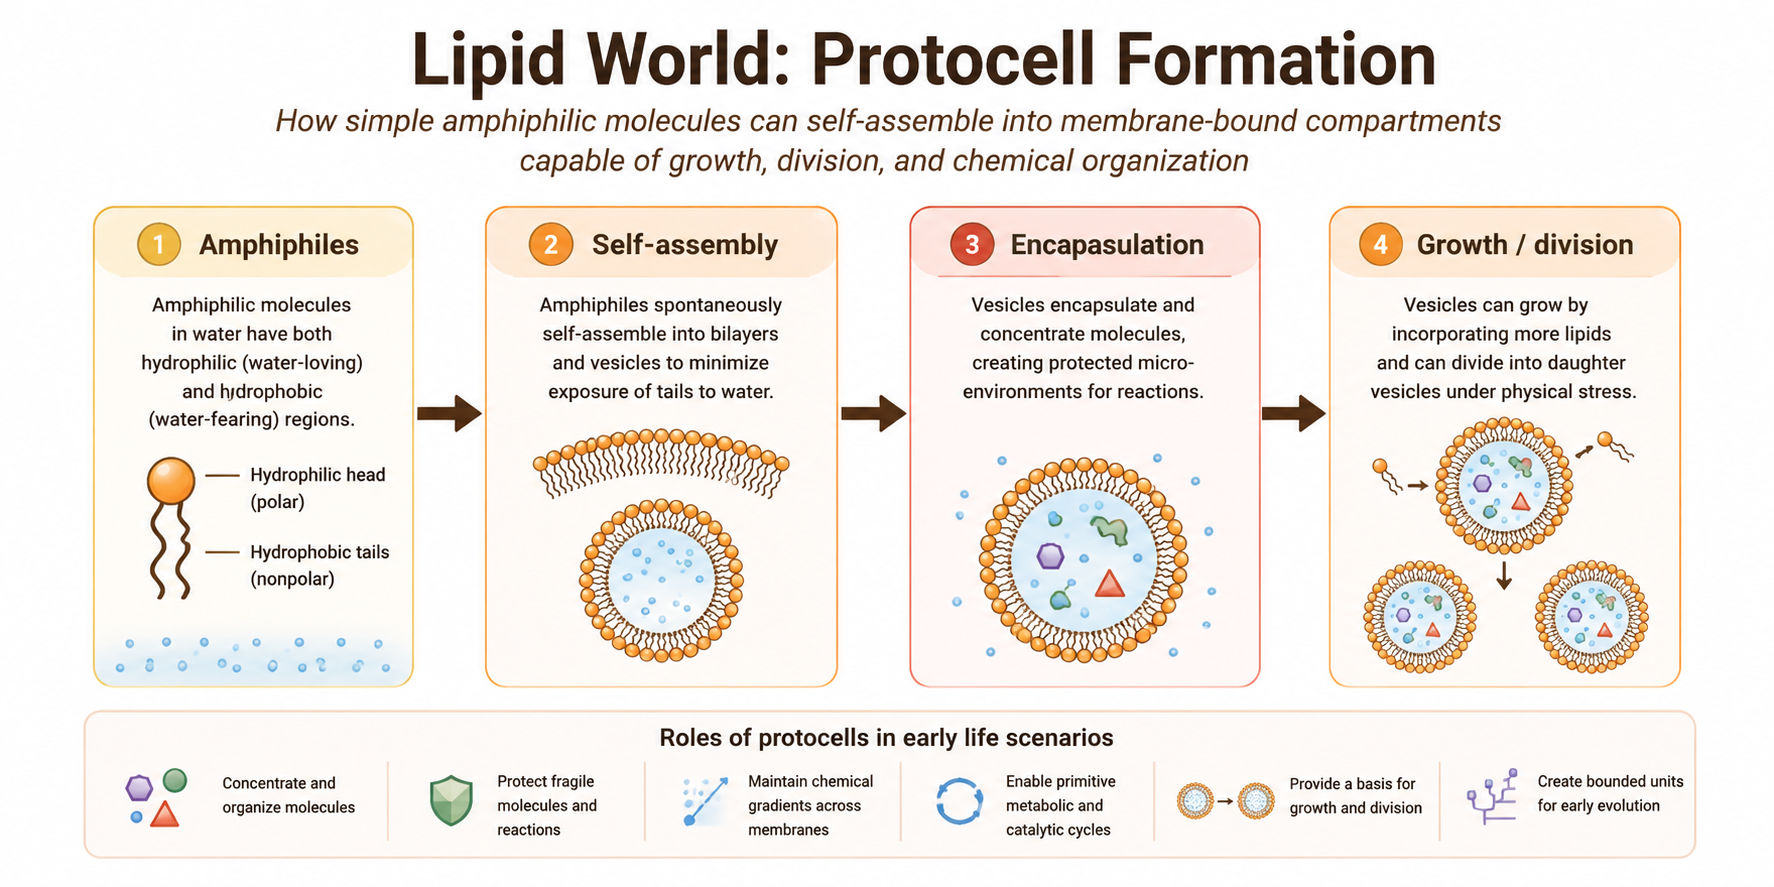
\includegraphics[width=1\linewidth]{figures/06_lipid_vesicle_formation} 

}

\caption{Conceptual mechanism of lipid world and protocell theories.}\label{fig:lipid-world-overview}
\end{figure}

The figure illustrates how simple amphiphilic molecules may have spontaneously self-assembled into membrane-bound structures capable of concentrating and stabilizing increasingly complex prebiotic chemistry.

Unlike metabolism-first or RNA-centered theories, lipid world models primarily address the emergence of physical compartmentalization.

\section{Protocell Formation}\label{protocell-formation}

Protocells represent one of the most important transitional concepts in origin-of-life research because they provide a possible bridge between chemistry and cellular organization.

Primitive protocells may have:
- Encapsulated organic molecules
- Concentrated catalytic reactions
- Maintained chemical gradients
- Protected fragile polymers
- Supported localized evolutionary processes

Some experimental studies demonstrate that fatty acid vesicles can:
- Grow by incorporating additional lipids
- Divide under physical stress
- Encapsulate nucleic acids
- Permit selective molecular transport

These behaviors resemble simplified versions of properties associated with living cells.

However, protocells remained chemically simple compared with modern biological cells and likely lacked sophisticated genetic control systems.

\section{Environmental Settings}\label{environmental-settings}

Several environments may have supported protocell formation under early Earth conditions:

\begin{itemize}
\tightlist
\item
  Tidal pools
\item
  Shoreline environments
\item
  Volcanic ponds
\item
  Hydrothermal regions
\item
  Wet--dry cycling environments
\end{itemize}

Wet--dry cycles are considered particularly important because repeated evaporation and hydration may promote membrane formation, vesicle fusion, and molecular encapsulation.

Environmental fluctuations may therefore have played a major role in protocell dynamics and membrane evolution.

\section{What the Theory Explains Well}\label{what-the-theory-explains-well-3}

Lipid world theories are particularly strong at explaining:

\begin{itemize}
\tightlist
\item
  Compartment formation
\item
  Molecular concentration
\item
  Physical organization of chemistry
\item
  Primitive selective boundaries
\item
  Encapsulation of reactions
\item
  Stabilization of prebiotic systems
\end{itemize}

Compartmentalization is considered essential because biological evolution requires organized systems capable of maintaining internal chemistry distinct from the surrounding environment.

Modern cells universally depend on membranes, suggesting that compartment formation was likely a critical transition during abiogenesis.

\section{What Makes It Plausible}\label{what-makes-it-plausible-3}

Several observations support the plausibility of lipid world theories:

\begin{itemize}
\tightlist
\item
  Amphiphilic molecules self-assemble spontaneously in water
\item
  Fatty acid vesicles form under experimentally realistic conditions
\item
  Membranes can encapsulate nucleic acids and catalysts
\item
  Vesicles can grow and divide under physical forces
\item
  Membrane structures occur naturally in modern biology
\end{itemize}

These findings suggest that compartment formation may emerge naturally from basic physical and chemical principles.

\section{Key Experimental and Observational Support}\label{key-experimental-and-observational-support-3}

Laboratory experiments demonstrate that fatty acids and related amphiphilic molecules readily form vesicles and bilayer membranes under plausible prebiotic conditions (\citeproc{ref-deamer2012}{Deamer 2012}).

Experimental protocells have also shown:
- Vesicle growth
- Membrane fusion
- Encapsulation of polymers
- Primitive transport behavior

Some studies suggest that mineral surfaces and wet--dry cycles may further enhance protocell formation and membrane stability.

Although these experiments do not recreate living cells, they strongly support the feasibility of spontaneous compartment formation.

\section{Major Gaps and Critiques}\label{major-gaps-and-critiques-3}

Despite their strengths, lipid world theories face several major limitations.

Most importantly, membrane formation alone does not explain:
- Heredity
- Replication
- Complex metabolism
- Information storage

Additional challenges include:
- Membrane instability under some environmental conditions
- Difficulty coordinating metabolism and heredity within protocells
- Limited catalytic capability of simple lipid systems
- Uncertainty regarding how protocells transitioned into fully living cells

For these reasons, protocell theories are generally viewed as necessary but incomplete components of abiogenesis.

\section{Integration with Other Theories}\label{integration-with-other-theories-3}

Lipid world theories integrate naturally with several other origin-of-life models.

Primitive membranes may have:
- Encapsulated RNA molecules
- Stabilized metabolic networks
- Maintained proton gradients
- Concentrated catalytic molecules
- Supported localized evolution

In many modern hybrid frameworks:
- Primordial synthesis produces organic molecules
- Metabolism-first models provide energy organization
- RNA World introduces heredity
- Lipid world theories provide compartmentalization

Together, these mechanisms may have contributed sequentially or simultaneously to the emergence of cellular life.

\section{Systems Perspective}\label{systems-perspective-3}

Within the comparative framework of this book, lipid world theories primarily address the emergence of compartmentalization and cellular organization.

Their greatest strength lies in explaining how early chemistry may have become spatially organized and protected from environmental dilution.

However, these theories do not independently explain heredity or fully developed metabolism. Consequently, protocell models are best understood as one component within larger systems-level explanations of life's emergence.

\section{Modern Relevance}\label{modern-relevance-3}

Lipid world and protocell research remain highly active fields within:
- Origin-of-life studies
- Synthetic biology
- Systems chemistry
- Astrobiology

Artificial protocell experiments are increasingly used to investigate minimal requirements for cellular behavior and self-organization.

Because membrane self-assembly depends on universal physical principles, protocell formation may also be relevant to the search for extraterrestrial life.

\section{Current Scientific Standing}\label{current-scientific-standing-3}

Lipid world and protocell theories remain influential components of modern abiogenesis research. Although they are rarely viewed as complete standalone explanations, they are widely considered essential for understanding how prebiotic chemistry may have become compartmentalized and increasingly cell-like.

Modern origin-of-life research increasingly integrates protocell formation with RNA-based heredity, geochemical energy systems, and environmental cycling mechanisms.

\section{Comparative Assessment}\label{comparative-assessment-3}

\begin{longtable}[]{@{}
  >{\raggedright\arraybackslash}p{(\columnwidth - 2\tabcolsep) * \real{0.5000}}
  >{\raggedright\arraybackslash}p{(\columnwidth - 2\tabcolsep) * \real{0.5000}}@{}}
\toprule\noalign{}
\begin{minipage}[b]{\linewidth}\raggedright
Dimension
\end{minipage} & \begin{minipage}[b]{\linewidth}\raggedright
Assessment
\end{minipage} \\
\midrule\noalign{}
\endhead
\bottomrule\noalign{}
\endlastfoot
Primary Contribution & Compartmentalization and protocell formation \\
Explanatory Strength & Strong for membrane organization \\
Mechanistic Plausibility & High \\
Experimental Support & Strong \\
Environmental Realism & Moderate to high \\
Main Limitation & Weak explanation for heredity and metabolism \\
Integrative Potential & Very high \\
Current Scientific Standing & Essential but incomplete component of abiogenesis models \\
\end{longtable}

\section{Comparative Performance}\label{comparative-performance-3}

\begin{longtable}[]{@{}ll@{}}
\toprule\noalign{}
Question & Lipid World Performance \\
\midrule\noalign{}
\endhead
\bottomrule\noalign{}
\endlastfoot
Produces organic building blocks? & Weak \\
Explains organized chemistry? & Moderate \\
Explains heredity? & Weak \\
Explains metabolism? & Weak--moderate \\
Explains compartment formation? & Strong \\
Supported experimentally? & Strong \\
Useful in hybrid models? & Very strong \\
\end{longtable}

\chapter{Warm Little Pond and Wet--Dry Cycle Theories}\label{warm-little-pond-and-wetdry-cycle-theories}

\section{Chapter Overview}\label{chapter-overview-4}

This chapter examines warm little pond and wet--dry cycle theories, which propose that fluctuating environmental conditions on early Earth may have promoted the concentration, polymerization, and organization of prebiotic molecules.

Unlike models centered primarily on heredity or metabolism, wet--dry cycle theories emphasize the importance of environmental cycling. Repeated hydration and dehydration may have provided natural physical mechanisms capable of concentrating dilute molecules, driving condensation reactions, and promoting increasingly complex prebiotic chemistry.

The chapter reviews the historical development of these ideas, the physical and chemical principles underlying wet--dry cycling, experimental evidence for polymer formation, major limitations, and the role of environmental cycling within broader hybrid models of abiogenesis.

\section{Key Terms}\label{key-terms-4}

\begin{itemize}
\tightlist
\item
  Warm little pond
\item
  Wet--dry cycles
\item
  Polymerization
\item
  Condensation reactions
\item
  Evaporation
\item
  Dehydration synthesis
\item
  Prebiotic concentration
\item
  Environmental cycling
\item
  Protochemistry
\end{itemize}

\section{Core Idea}\label{core-idea-4}

Warm little pond and wet--dry cycle theories propose that shallow surface environments on early Earth may have provided ideal conditions for concentrating organic molecules and promoting increasingly complex chemical reactions.

In dilute aqueous environments, prebiotic molecules are often too dispersed to react efficiently. However, repeated cycles of evaporation and rehydration can dramatically increase local concentrations and promote chemical bonding reactions.

These environmental cycles may therefore have helped bridge the gap between simple organic molecules and larger polymers such as peptides, nucleic acid chains, and primitive catalytic networks.

Charles Darwin famously speculated that life may have originated in a ``warm little pond,'' though modern versions of the theory incorporate a far more sophisticated understanding of prebiotic chemistry and environmental dynamics.

\section{Historical Context}\label{historical-context-4}

Interest in wet--dry cycling emerged partly in response to challenges faced by primordial soup and hydrothermal vent models.

Open ocean environments present major dilution problems for prebiotic chemistry because organic molecules become widely dispersed in large water volumes. In contrast, shallow ponds, volcanic pools, geothermal fields, and periodically drying environments naturally concentrate dissolved compounds.

Researchers including David Deamer and Bruce Damer proposed that repeated wet--dry cycling may have played a critical role in polymer formation, membrane assembly, and protocell emergence under realistic early Earth conditions (\citeproc{ref-deamer2012}{Deamer 2012}).

These ideas are now considered important components of many modern hybrid origin-of-life frameworks.

\section{Mechanistic Basis}\label{mechanistic-basis-4}

Wet--dry cycle theories rely on a simple but powerful environmental mechanism:

\begin{enumerate}
\def\labelenumi{\arabic{enumi}.}
\tightlist
\item
  Molecules accumulate in shallow aqueous environments
\item
  Evaporation concentrates dissolved compounds
\item
  Dehydration promotes condensation reactions
\item
  Rehydration redistributes products
\item
  Repeated cycling increases chemical complexity
\end{enumerate}

During drying phases:
- Water activity decreases
- Molecules become concentrated
- Condensation reactions become thermodynamically favorable
- Polymer formation may occur more readily

During rehydration phases:
- Molecules become mobile again
- Vesicles may reform
- Products can redistribute and interact
- Selection-like processes may emerge

Figure \ref{fig:warm-little-pond-overview} summarizes the conceptual mechanism proposed by warm little pond and wet--dry cycle theories.

\begin{figure}

{\centering 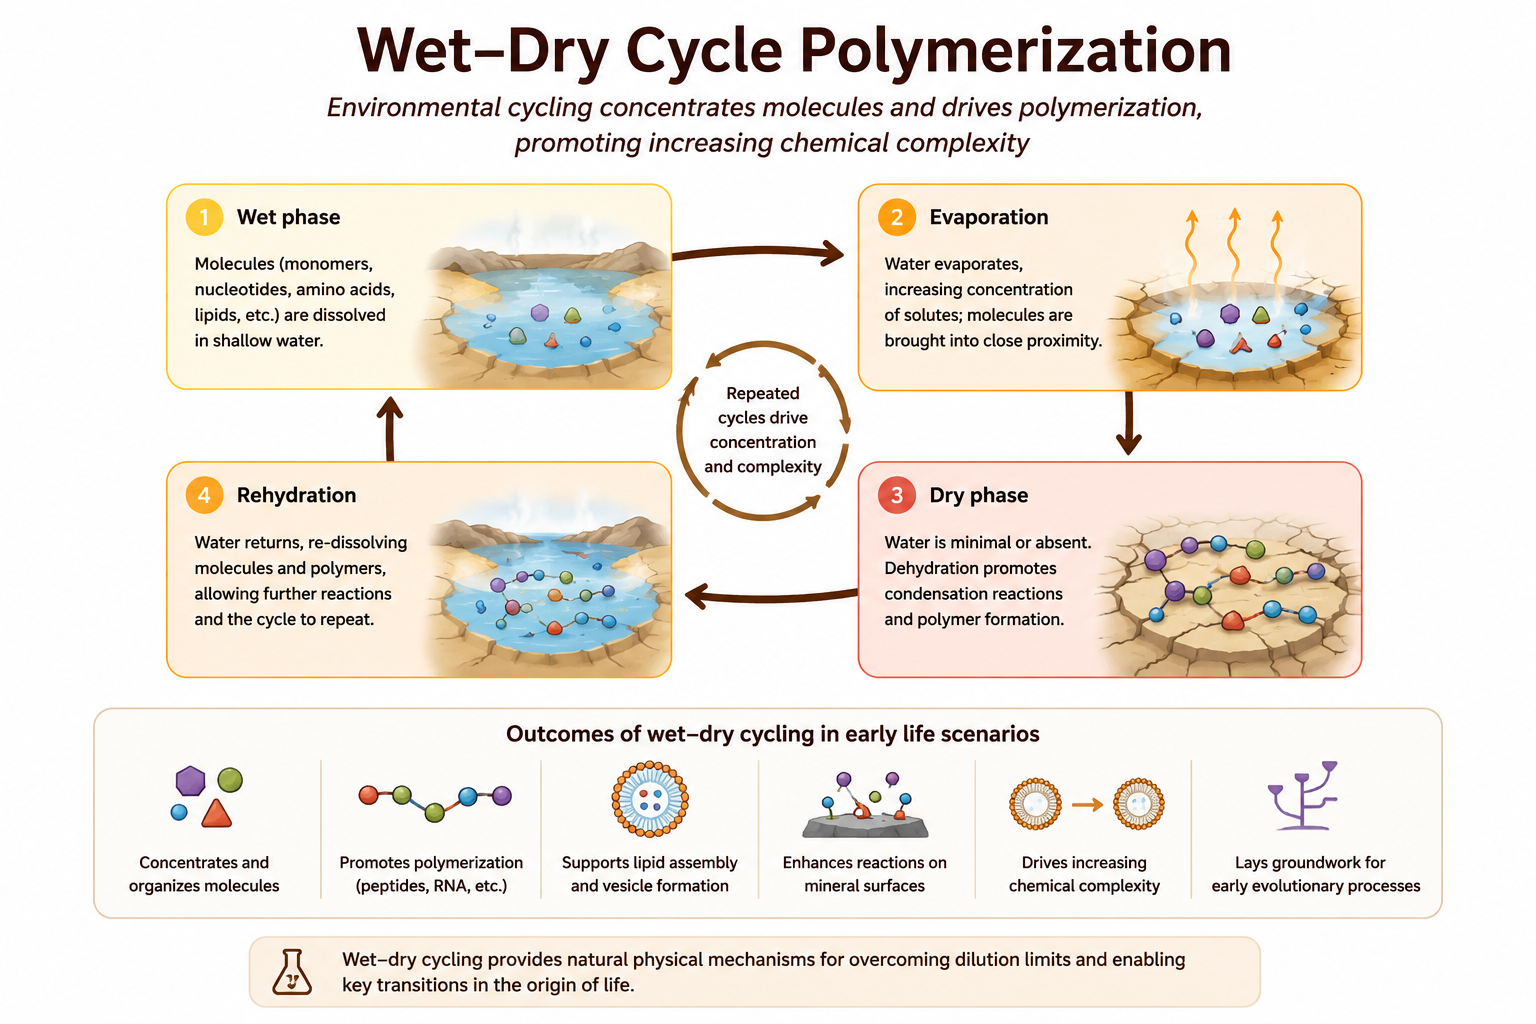
\includegraphics[width=1\linewidth]{figures/07_wet_dry_cycle_polymerization} 

}

\caption{Conceptual mechanism of warm little pond and wet–dry cycle theories.}\label{fig:warm-little-pond-overview}
\end{figure}

The figure illustrates how environmental cycling may have promoted concentration, polymerization, membrane assembly, and increasingly complex prebiotic chemistry.

Unlike purely chemical synthesis models, wet--dry cycle theories emphasize the dynamic interaction between chemistry and environmental fluctuation.

\section{Polymerization and Chemical Complexity}\label{polymerization-and-chemical-complexity}

One of the most important contributions of wet--dry cycle models is their ability to explain polymer formation under plausible early Earth conditions.

Many biologically important molecules form through condensation reactions that release water, including:
- Peptide formation
- Ester formation
- Phosphodiester bond formation

These reactions are generally unfavorable in continuously wet environments because excess water drives the reactions backward.

Drying conditions may therefore have provided a natural mechanism for:
- Peptide synthesis
- RNA-like polymer formation
- Lipid assembly
- Proto-metabolic organization

Repeated environmental cycling could gradually increase molecular complexity over time.

\section{Environmental Settings}\label{environmental-settings-1}

Several early Earth environments may have supported wet--dry cycling:

\begin{itemize}
\tightlist
\item
  Volcanic geothermal fields
\item
  Tidal pools
\item
  Hot spring systems
\item
  Seasonal ponds
\item
  Shoreline environments
\item
  Impact-generated hydrothermal systems
\end{itemize}

Geothermal environments are considered particularly important because they provide:
- Heat
- Mineral surfaces
- Chemical gradients
- Intermittent hydration
- Repeated environmental cycling

Mineral surfaces may also enhance concentration and catalysis during drying phases.

\section{Relationship with Other Theories}\label{relationship-with-other-theories}

Wet--dry cycle theories integrate naturally with several other origin-of-life models.

Environmental cycling may support:
- Primordial soup chemistry
- RNA polymerization
- Lipid vesicle formation
- Mineral surface catalysis
- Proto-metabolic reactions

In many hybrid frameworks:
- Primordial synthesis produces organic precursors
- Wet--dry cycles concentrate and polymerize molecules
- Lipid membranes form protocells
- RNA systems introduce heredity

Thus, environmental cycling may act as an important organizing mechanism linking multiple origin-of-life processes.

\section{What the Theory Explains Well}\label{what-the-theory-explains-well-4}

Warm little pond and wet--dry cycle theories are particularly strong at explaining:

\begin{itemize}
\tightlist
\item
  Molecular concentration
\item
  Polymerization
\item
  Environmental organization
\item
  Condensation reactions
\item
  Repeated chemical cycling
\item
  Increased molecular complexity
\end{itemize}

These theories provide plausible physical mechanisms for overcoming dilution problems that affect many prebiotic chemistry models.

They also naturally integrate environmental variability into abiogenesis research.

\section{What Makes It Plausible}\label{what-makes-it-plausible-4}

Several observations support the plausibility of wet--dry cycle theories:

\begin{itemize}
\tightlist
\item
  Evaporation naturally concentrates solutes
\item
  Condensation reactions occur more readily during dehydration
\item
  Experimental wet--dry cycles promote polymer formation
\item
  Geothermal fields likely existed on early Earth
\item
  Environmental cycling remains common in modern Earth systems
\end{itemize}

The theory is also attractive because it relies on ordinary physical processes rather than highly specialized assumptions.

\section{Key Experimental and Observational Support}\label{key-experimental-and-observational-support-4}

Experimental studies demonstrate that wet--dry cycling can promote:
- Peptide synthesis
- RNA-like polymerization
- Vesicle formation
- Molecular encapsulation
- Increased chemical complexity

Some laboratory studies show that repeated dehydration and rehydration cycles can generate surprisingly complex molecular systems under plausible prebiotic conditions (\citeproc{ref-deamer2012}{Deamer 2012}).

Geological evidence also suggests that volcanic and geothermal environments were widespread on early Earth.

\section{Major Gaps and Critiques}\label{major-gaps-and-critiques-4}

Despite its strengths, the theory faces several important limitations.

Major unresolved questions include:
- Stability of polymers under harsh conditions
- Transition from polymers to heredity
- Long-term persistence of prebiotic systems
- Integration with metabolism
- Environmental realism of some experimental conditions

Additional criticism concerns the difficulty of demonstrating how wet--dry cycling alone could generate self-replicating systems or fully organized protocells.

Consequently, most researchers view wet--dry cycle theories as partial rather than complete explanations.

\section{Systems Perspective}\label{systems-perspective-4}

Within the comparative framework of this book, warm little pond and wet--dry cycle theories primarily address environmental concentration and polymerization.

Their greatest strength lies in explaining how fluctuating environmental conditions may have driven increasingly complex chemistry under realistic early Earth settings.

However, these theories do not independently explain:
- Stable heredity
- Advanced metabolism
- Darwinian evolution

For this reason, they are generally viewed as complementary components within larger systems-level models of abiogenesis.

\section{Modern Relevance}\label{modern-relevance-4}

Wet--dry cycle research remains highly influential in:
- Prebiotic chemistry
- Systems chemistry
- Astrobiology
- Geochemistry
- Synthetic protocell research

Modern work increasingly explores how environmental cycling may interact with:
- Mineral catalysis
- Membrane assembly
- RNA systems
- Energy gradients

Because fluctuating environments may occur on other planetary bodies, wet--dry cycle theories are also relevant to astrobiology and the search for extraterrestrial life.

\section{Current Scientific Standing}\label{current-scientific-standing-4}

Warm little pond and wet--dry cycle theories remain influential and actively studied components of modern origin-of-life research. Although they are rarely viewed as complete standalone explanations, they are widely considered plausible mechanisms for overcoming dilution barriers and promoting polymerization under realistic environmental conditions.

Many current hybrid models incorporate wet--dry cycling as a key organizational mechanism linking prebiotic synthesis, polymer formation, and protocell assembly.

\section{Comparative Assessment}\label{comparative-assessment-4}

\begin{longtable}[]{@{}
  >{\raggedright\arraybackslash}p{(\columnwidth - 2\tabcolsep) * \real{0.5000}}
  >{\raggedright\arraybackslash}p{(\columnwidth - 2\tabcolsep) * \real{0.5000}}@{}}
\toprule\noalign{}
\begin{minipage}[b]{\linewidth}\raggedright
Dimension
\end{minipage} & \begin{minipage}[b]{\linewidth}\raggedright
Assessment
\end{minipage} \\
\midrule\noalign{}
\endhead
\bottomrule\noalign{}
\endlastfoot
Primary Contribution & Concentration and polymerization \\
Explanatory Strength & Strong for environmental organization \\
Mechanistic Plausibility & High \\
Experimental Support & Strong \\
Environmental Realism & Moderate to high \\
Main Limitation & Weak explanation for heredity \\
Integrative Potential & Very high \\
Current Scientific Standing & Important component of hybrid abiogenesis models \\
\end{longtable}

\section{Comparative Performance}\label{comparative-performance-4}

\begin{longtable}[]{@{}ll@{}}
\toprule\noalign{}
Question & Wet--Dry Cycle Performance \\
\midrule\noalign{}
\endhead
\bottomrule\noalign{}
\endlastfoot
Produces organic building blocks? & Moderate \\
Explains concentration mechanisms? & Strong \\
Explains polymerization? & Strong \\
Explains heredity? & Weak \\
Explains metabolism? & Weak--moderate \\
Supported experimentally? & Strong \\
Useful in hybrid models? & Very strong \\
\end{longtable}

\chapter{Clay and Mineral Template Hypotheses}\label{clay-and-mineral-template-hypotheses}

\section{Chapter Overview}\label{chapter-overview-5}

This chapter examines clay and mineral template hypotheses, which propose that mineral surfaces on early Earth may have played a central role in organizing, concentrating, and catalyzing prebiotic chemistry.

Unlike theories focused primarily on heredity, metabolism, or compartment formation, mineral template models emphasize the importance of solid surfaces as physical and chemical scaffolds for molecular organization. Certain minerals may have promoted adsorption, alignment, polymerization, and stabilization of organic molecules under realistic prebiotic conditions.

The chapter reviews the historical development of mineral-template theories, the mechanisms by which mineral surfaces influence chemical reactions, experimental evidence for surface-catalyzed polymerization, major limitations, and the role of minerals within broader hybrid models of abiogenesis.

\section{Key Terms}\label{key-terms-5}

\begin{itemize}
\tightlist
\item
  Clay minerals
\item
  Mineral templates
\item
  Surface catalysis
\item
  Adsorption
\item
  Montmorillonite
\item
  Prebiotic polymerization
\item
  Chemical scaffolding
\item
  Surface chemistry
\item
  Mineral-assisted organization
\end{itemize}

\section{Core Idea}\label{core-idea-5}

Clay and mineral template hypotheses propose that mineral surfaces may have acted as natural catalytic and organizational platforms during the origin of life.

In aqueous environments, organic molecules are often highly diluted and randomly distributed. Mineral surfaces can partially overcome this problem by adsorbing molecules onto structured solid interfaces where they become concentrated and spatially organized.

This organization may promote:
- Chemical reactions
- Polymer formation
- Molecular alignment
- Stabilization of intermediates
- Primitive catalytic networks

Some minerals may therefore have functioned as primitive templates that guided increasingly complex chemistry before the emergence of fully biological systems.

\section{Historical Context}\label{historical-context-5}

Interest in mineral-assisted prebiotic chemistry developed partly in response to challenges faced by purely solution-based origin-of-life models.

Researchers recognized that mineral surfaces naturally:
- Concentrate molecules
- Provide catalytic sites
- Stabilize reactive intermediates
- Create structured microenvironments

A major development came from the work of A. G. Cairns-Smith, who proposed that clay crystals themselves may have participated in primitive information transfer and selection processes.

Later experimental work demonstrated that minerals such as montmorillonite clay can catalyze RNA-like polymerization reactions under laboratory conditions (\citeproc{ref-ferris2006}{Ferris 2006}).

These findings increased scientific interest in the possible role of minerals as early organizational scaffolds.

\section{Mechanistic Basis}\label{mechanistic-basis-5}

Mineral template hypotheses are based on interactions between dissolved organic molecules and structured mineral surfaces.

Key mechanisms include:

\begin{itemize}
\tightlist
\item
  Adsorption of molecules onto mineral surfaces
\item
  Surface concentration of reactants
\item
  Alignment of molecules into reactive orientations
\item
  Catalysis of bond formation
\item
  Stabilization of polymers and intermediates
\end{itemize}

Certain clay minerals possess layered structures and charged surfaces that can attract and organize organic molecules.

Figure \ref{fig:clay-mineral-overview} summarizes the conceptual mechanism proposed by clay and mineral template hypotheses.

\begin{figure}

{\centering 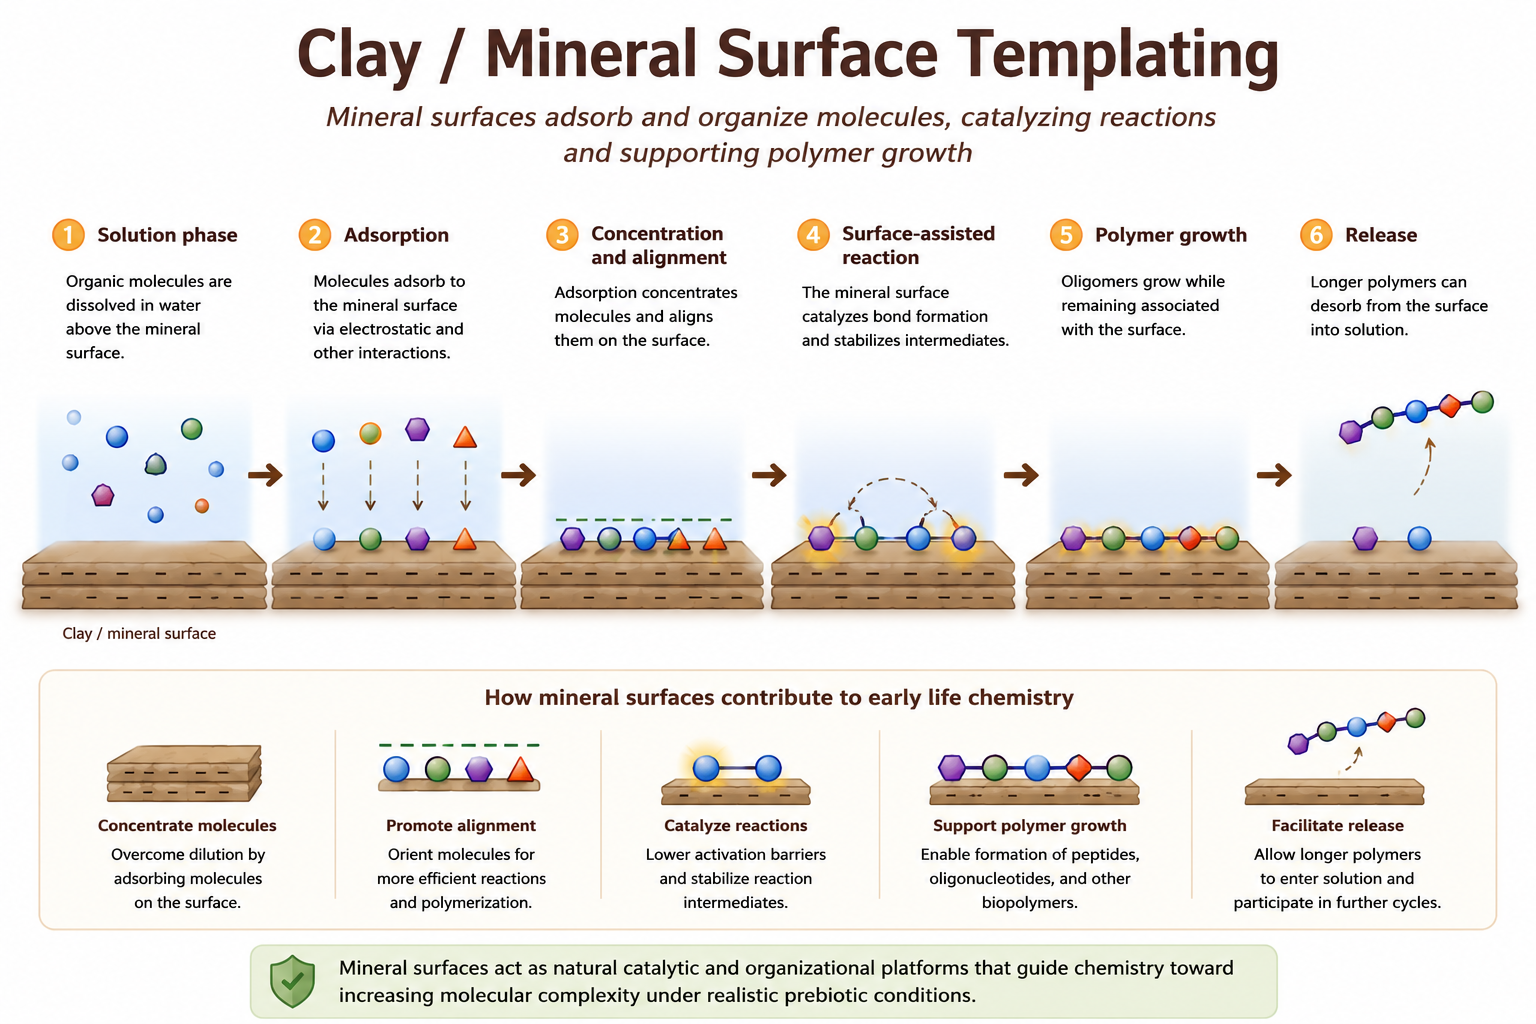
\includegraphics[width=1\linewidth]{figures/08_clay_mineral_template} 

}

\caption{Conceptual mechanism of clay and mineral template hypotheses.}\label{fig:clay-mineral-overview}
\end{figure}

The figure illustrates how mineral surfaces may have concentrated molecules, promoted polymerization, and supported increasingly organized prebiotic chemistry.

Unlike purely aqueous chemistry models, mineral-template theories emphasize the importance of structured physical surfaces in guiding chemical evolution.

\section{Mineral Surfaces and Prebiotic Chemistry}\label{mineral-surfaces-and-prebiotic-chemistry}

Minerals may have influenced prebiotic chemistry in several important ways.

\subsection{Concentration of Molecules}\label{concentration-of-molecules}

Adsorption onto mineral surfaces can locally increase molecular concentration, helping overcome dilution problems present in open aqueous environments.

\subsection{Molecular Alignment}\label{molecular-alignment}

Surface structures may orient molecules into favorable geometries for chemical reactions and polymer formation.

\subsection{Catalysis}\label{catalysis}

Some minerals possess catalytic properties capable of promoting:
- Condensation reactions
- Polymerization
- Redox reactions
- Bond stabilization

\subsection{Protection and Stabilization}\label{protection-and-stabilization}

Mineral surfaces may protect fragile molecules from:
- Hydrolysis
- UV radiation
- Environmental disruption

These combined effects make minerals attractive candidates for supporting early chemical organization.

\section{Important Mineral Candidates}\label{important-mineral-candidates}

Several minerals are commonly discussed in origin-of-life research:

\begin{itemize}
\tightlist
\item
  Montmorillonite clay
\item
  Iron--sulfur minerals
\item
  Pyrite surfaces
\item
  Silicate minerals
\item
  Metal sulfides
\end{itemize}

Montmorillonite is especially important because experiments demonstrate that it can catalyze the formation of RNA-like oligomers from activated nucleotides.

Iron--sulfur minerals are also closely connected with metabolism-first and hydrothermal vent theories.

\section{Relationship with Other Theories}\label{relationship-with-other-theories-1}

Mineral-template theories integrate naturally with several other abiogenesis models.

Mineral surfaces may support:
- Primordial soup chemistry
- RNA polymerization
- Wet--dry cycle chemistry
- Lipid assembly
- Proto-metabolic reactions

In many hybrid frameworks:
- Primordial synthesis generates organic molecules
- Mineral surfaces organize and catalyze reactions
- Wet--dry cycles promote polymerization
- Protocells provide compartmentalization
- RNA systems introduce heredity

Thus, minerals may have acted as physical scaffolds linking multiple stages of prebiotic evolution.

\section{What the Theory Explains Well}\label{what-the-theory-explains-well-5}

Clay and mineral template hypotheses are particularly strong at explaining:

\begin{itemize}
\tightlist
\item
  Spatial organization of molecules
\item
  Surface catalysis
\item
  Concentration mechanisms
\item
  Polymer alignment
\item
  Reaction scaffolding
\item
  Enhanced polymerization
\end{itemize}

These theories provide plausible physical mechanisms for organizing prebiotic chemistry under realistic geological conditions.

\section{What Makes It Plausible}\label{what-makes-it-plausible-5}

Several observations support the plausibility of mineral-template models:

\begin{itemize}
\tightlist
\item
  Mineral surfaces naturally occur on Earth
\item
  Many minerals adsorb organic molecules
\item
  Surface catalysis is common in chemistry
\item
  Clay minerals promote polymerization experimentally
\item
  Minerals provide stable microenvironments
\end{itemize}

The theory is attractive because it relies on ordinary geological processes that likely existed on the early Earth.

\section{Key Experimental and Observational Support}\label{key-experimental-and-observational-support-5}

Laboratory experiments demonstrate that clay minerals such as montmorillonite can catalyze the formation of RNA-like oligomers from activated nucleotides (\citeproc{ref-ferris2006}{Ferris 2006}).

Additional studies show that minerals can:
- Concentrate organic molecules
- Promote vesicle assembly
- Catalyze condensation reactions
- Stabilize polymers

Geological evidence also indicates that clay-rich and mineral-rich environments were widespread on the early Earth.

\section{Major Gaps and Critiques}\label{major-gaps-and-critiques-5}

Despite their strengths, mineral-template theories face several important limitations.

Major unresolved questions include:
- Transition from surface-bound chemistry to free-living systems
- Emergence of heredity
- Development of autonomous metabolism
- Transfer of information away from mineral templates
- Environmental realism of some experimental conditions

Critics also argue that mineral surfaces alone do not explain:
- Self-replication
- Cellular organization
- Darwinian evolution

Consequently, most researchers view mineral-template theories as partial rather than complete explanations of abiogenesis.

\section{Systems Perspective}\label{systems-perspective-5}

Within the comparative framework of this book, clay and mineral template hypotheses primarily address chemical organization and catalysis.

Their greatest strength lies in explaining how structured physical environments may have guided increasingly complex chemistry before the emergence of fully biological systems.

However, these theories do not independently explain:
- Stable heredity
- Cellular compartmentalization
- Fully developed metabolism

For this reason, mineral-template models are generally treated as complementary components within broader systems-level origin-of-life frameworks.

\section{Modern Relevance}\label{modern-relevance-5}

Mineral-template research remains highly influential in:
- Prebiotic chemistry
- Surface chemistry
- Geochemistry
- Systems chemistry
- Astrobiology

Modern studies increasingly examine how mineral surfaces interact with:
- RNA systems
- Lipid membranes
- Wet--dry cycles
- Hydrothermal chemistry

Because minerals are abundant throughout the Solar System, these theories are also relevant to the search for extraterrestrial life.

\section{Current Scientific Standing}\label{current-scientific-standing-5}

Clay and mineral template hypotheses remain influential and actively studied components of modern origin-of-life research. Although they are rarely viewed as complete standalone explanations, they are widely considered plausible mechanisms for organizing and catalyzing increasingly complex prebiotic chemistry.

Many current hybrid models incorporate mineral surfaces as important environmental scaffolds linking chemistry, polymerization, and early molecular organization.

\section{Comparative Assessment}\label{comparative-assessment-5}

\begin{longtable}[]{@{}
  >{\raggedright\arraybackslash}p{(\columnwidth - 2\tabcolsep) * \real{0.5000}}
  >{\raggedright\arraybackslash}p{(\columnwidth - 2\tabcolsep) * \real{0.5000}}@{}}
\toprule\noalign{}
\begin{minipage}[b]{\linewidth}\raggedright
Dimension
\end{minipage} & \begin{minipage}[b]{\linewidth}\raggedright
Assessment
\end{minipage} \\
\midrule\noalign{}
\endhead
\bottomrule\noalign{}
\endlastfoot
Primary Contribution & Molecular organization and surface catalysis \\
Explanatory Strength & Strong for spatial organization \\
Mechanistic Plausibility & Moderate--high \\
Experimental Support & Moderate--strong \\
Environmental Realism & Moderate \\
Main Limitation & Weak explanation for autonomy and heredity \\
Integrative Potential & Very high \\
Current Scientific Standing & Important component of hybrid abiogenesis models \\
\end{longtable}

\section{Comparative Performance}\label{comparative-performance-5}

\begin{longtable}[]{@{}ll@{}}
\toprule\noalign{}
Question & Clay/Mineral Template Performance \\
\midrule\noalign{}
\endhead
\bottomrule\noalign{}
\endlastfoot
Produces organic building blocks? & Weak \\
Explains concentration mechanisms? & Strong \\
Explains polymerization? & Moderate--strong \\
Explains heredity? & Weak \\
Explains metabolism? & Weak--moderate \\
Supported experimentally? & Moderate--strong \\
Useful in hybrid models? & Very strong \\
\end{longtable}

\chapter{Protein-First and Peptide World Theories}\label{protein-first-and-peptide-world-theories}

\section{Chapter Overview}\label{chapter-overview-6}

This chapter examines protein-first and peptide world theories, which propose that short peptides may have played important catalytic roles before the emergence of nucleic-acid heredity. The chapter reviews the proposed mechanism, supporting evidence, limitations, and the role of peptides within broader hybrid models of abiogenesis.

\section{Core Idea}\label{core-idea-6}

Protein-first and peptide world theories propose that simple peptides may have acted as primitive catalysts before nucleic-acid heredity emerged. In these models, catalytic chemistry preceded true genetic systems, allowing increasingly complex reaction networks to develop under prebiotic conditions.

Rather than beginning with informational molecules such as RNA, these theories suggest that early life may initially have depended on functional chemistry and primitive catalysis.

\section{Key Terms}\label{key-terms-6}

\begin{itemize}
\tightlist
\item
  Protein-first
\item
  Peptide world
\item
  Amino acids
\item
  Peptide bonds
\item
  Primitive catalysis
\item
  Metal-assisted catalysis
\item
  Reaction networks
\item
  Heredity
\end{itemize}

\section{Historical Context}\label{historical-context-6}

Protein-first theories emerged partly in response to limitations associated with purely RNA-centered origin-of-life models. Researchers questioned whether RNA molecules alone could realistically account for the earliest stages of chemical evolution without prior catalytic support.

Early work by Sidney Fox, Günter Wächtershäuser, and others proposed that amino acids and short peptides may have formed naturally on the early Earth and contributed to primitive metabolic organization before the emergence of hereditary systems.

These ideas became increasingly important after experimental studies demonstrated that amino acids form relatively easily under simulated prebiotic conditions.

\section{Mechanistic Basis}\label{mechanistic-basis-6}

Protein-first theories emphasize the catalytic potential of short peptides and amino-acid assemblies. The proposed pathway generally involves:

\begin{enumerate}
\def\labelenumi{\arabic{enumi}.}
\tightlist
\item
  Abiotic synthesis of amino acids
\item
  Peptide bond formation and short-chain assembly
\item
  Emergence of primitive catalytic activity
\item
  Stabilization of chemical reaction networks
\item
  Increasing molecular complexity prior to nucleic-acid heredity
\end{enumerate}

Figure \ref{fig:protein-first-mechanism} summarizes the conceptual mechanism proposed by peptide-world theories.

\begin{figure}
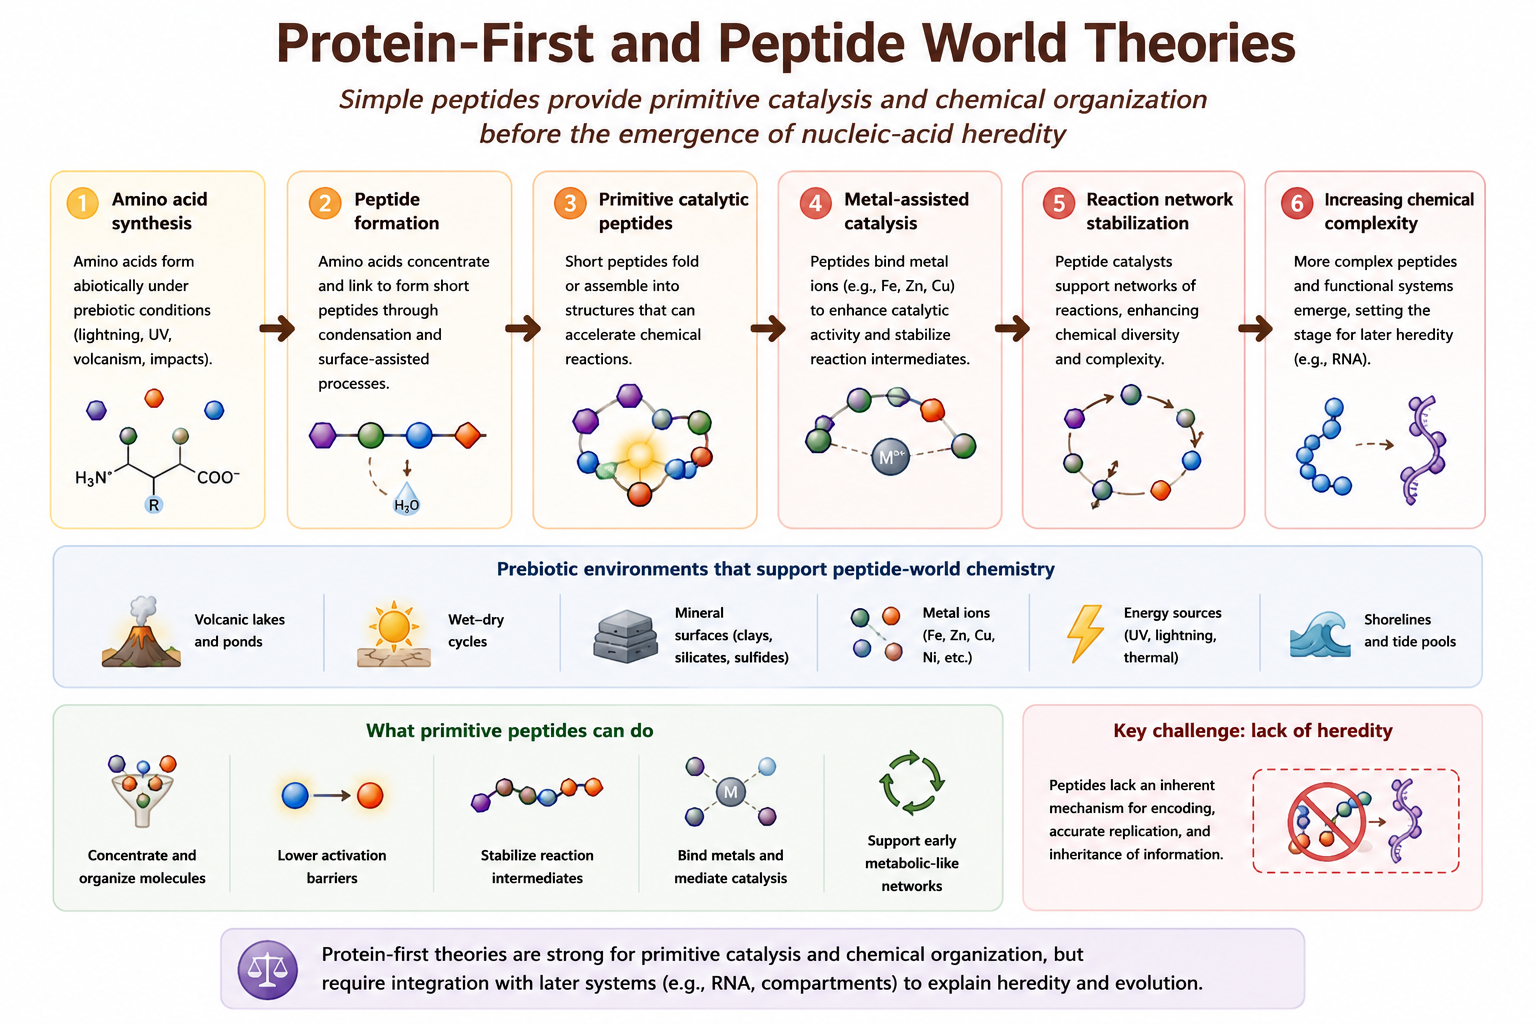
\includegraphics[width=1\linewidth]{figures/09_protein_first_mechanism} \caption{Conceptual mechanism of Protein-First and Peptide World theories. Primitive peptides may have supported early catalysis and chemical organization before nucleic-acid heredity emerged.}\label{fig:protein-first-mechanism}
\end{figure}

The figure illustrates how simple peptides may have contributed to early catalysis, energy transfer, and stabilization of reaction pathways before the development of true hereditary systems.

Many versions of the theory also emphasize the importance of metal ions and mineral surfaces in promoting peptide formation and catalytic activity.

\section{What the Theory Explains Well}\label{what-the-theory-explains-well-6}

Protein-first theories are strongest at explaining:

\begin{itemize}
\tightlist
\item
  Primitive catalysis
\item
  Reaction acceleration
\item
  Metal-assisted chemistry
\item
  Early metabolic organization
\item
  Functional chemistry before heredity
\end{itemize}

These models provide a plausible explanation for how increasingly complex chemical systems may have emerged before the appearance of sophisticated genetic replication.

\section{What Makes It Plausible}\label{what-makes-it-plausible-6}

Several observations support the plausibility of peptide-world scenarios:

\begin{itemize}
\tightlist
\item
  Amino acids form readily under simulated prebiotic conditions
\item
  Amino acids are detected in meteorites and interstellar chemistry
\item
  Short peptides can form through dehydration reactions
\item
  Small peptides can exhibit catalytic properties
\item
  Metal-peptide complexes may stabilize primitive reactions
\end{itemize}

Experimental studies also show that peptides may assist with membrane stabilization and molecular organization.

\section{Key Experimental and Observational Support}\label{key-experimental-and-observational-support-6}

Evidence supporting protein-first models includes:

\begin{itemize}
\tightlist
\item
  Miller--Urey-type amino acid synthesis experiments
\item
  Detection of amino acids in carbonaceous meteorites
\item
  Laboratory peptide polymerization experiments
\item
  Metal-binding peptide catalysis
\item
  Surface-assisted peptide assembly on minerals
\end{itemize}

Some experimental systems further suggest that wet--dry cycles may naturally promote peptide bond formation.

\section{Relationship to Other Origin-of-Life Theories}\label{relationship-to-other-origin-of-life-theories}

Protein-first theories overlap strongly with several other origin-of-life frameworks:

\begin{itemize}
\tightlist
\item
  Metabolism-first theories through catalytic reaction networks
\item
  Hydrothermal vent theories through metal-assisted chemistry
\item
  Wet--dry cycle theories through peptide polymerization
\item
  RNA world models through possible later integration with hereditary systems
\end{itemize}

Most modern researchers therefore view peptide-world models as complementary components within broader hybrid origin-of-life scenarios.

\section{Systems Perspective}\label{systems-perspective-6}

Within the comparative framework of this book, protein-first theories primarily address the emergence of primitive catalytic function. Their greatest strength lies in explaining how early reaction networks may have become faster, more selective, and more chemically organized.

However, peptides alone do not provide a clear mechanism for information storage, replication, or long-term inheritance. For this reason, protein-first theories are best understood as complementary to RNA-world, metabolism-first, mineral-template, and protocell models rather than as complete explanations of abiogenesis.

\section{Major Gaps and Critiques}\label{major-gaps-and-critiques-6}

The largest unresolved problem is heredity.

Unlike nucleic acids, peptides do not naturally provide a robust mechanism for encoded information storage or accurate template replication. As a result, protein-first systems struggle to explain how Darwinian evolution could begin without the later emergence of RNA or related informational molecules.

Additional challenges include:

\begin{itemize}
\tightlist
\item
  Limited replication fidelity
\item
  Weak evolutionary memory
\item
  Lack of stable inheritance mechanisms
\item
  Difficulty transitioning toward modern genetics
\end{itemize}

\section{Current Scientific Standing}\label{current-scientific-standing-6}

Protein-first theories remain scientifically important as partial explanations for early catalytic organization and prebiotic chemistry. However, they are rarely treated as complete standalone explanations for abiogenesis.

Most current research instead treats peptides as likely cooperative partners within broader hybrid models involving RNA, metabolism, mineral catalysis, and protocell formation.

\section{Comparative Assessment}\label{comparative-assessment-6}

\begin{longtable}[]{@{}
  >{\raggedright\arraybackslash}p{(\columnwidth - 2\tabcolsep) * \real{0.5000}}
  >{\raggedright\arraybackslash}p{(\columnwidth - 2\tabcolsep) * \real{0.5000}}@{}}
\toprule\noalign{}
\begin{minipage}[b]{\linewidth}\raggedright
Dimension
\end{minipage} & \begin{minipage}[b]{\linewidth}\raggedright
Assessment
\end{minipage} \\
\midrule\noalign{}
\endhead
\bottomrule\noalign{}
\endlastfoot
Primary Contribution & Primitive catalysis and reaction acceleration \\
Explanatory Strength & Strong for functional chemistry before heredity \\
Mechanistic Plausibility & Moderate \\
Experimental Support & Moderate \\
Environmental Realism & Moderate \\
Main Limitation & Lack of robust heredity and encoded information \\
Integrative Potential & High \\
Current Scientific Standing & Useful but incomplete supporting model \\
\end{longtable}

\section{Performance Across Major Abiogenesis Challenges}\label{performance-across-major-abiogenesis-challenges}

Table \ref{tab:protein-performance} summarizes how protein-first theories perform across the major origin-of-life transitions introduced earlier in this book.

\begin{table}

\caption{\label{tab:protein-performance}Comparative performance of Protein-First and Peptide World theories across major abiogenesis challenges.}
\centering
\begin{tabular}[t]{l|l}
\hline
Challenge & Performance\\
\hline
Abiotic synthesis & Strong\\
\hline
Catalysis & Strong\\
\hline
Metabolic organization & Moderate-Strong\\
\hline
Compartment formation & Weak\\
\hline
Information storage & Weak\\
\hline
Hereditary replication & Weak\\
\hline
Darwinian evolution & Limited\\
\hline
\end{tabular}
\end{table}

The strongest contribution of protein-first theories lies in their ability to explain primitive catalytic chemistry and early reaction networks. Their weakest area remains the emergence of stable hereditary information and long-term evolutionary memory.

\chapter{Panspermia and Lithopanspermia}\label{panspermia-and-lithopanspermia}

\section{Chapter Overview}\label{chapter-overview-7}

This chapter examines panspermia and lithopanspermia theories, which propose that life---or at least important prebiotic materials---may have originated elsewhere in space and later arrived on Earth through natural interplanetary transfer processes.

Unlike most abiogenesis theories, panspermia does not primarily explain how life first emerged. Instead, it focuses on whether microorganisms or prebiotic compounds could survive transfer between planetary bodies.

This chapter evaluates the physical plausibility of interplanetary transfer, microbial survival under extreme conditions, and the limitations of panspermia as a complete explanation for the origin of life.

\section{Core Idea}\label{core-idea-7}

Panspermia proposes that life, microorganisms, or prebiotic organic compounds may have been transferred to Earth from elsewhere in the Solar System or beyond.

Several forms of panspermia have been proposed:

\begin{itemize}
\tightlist
\item
  \textbf{Radiopanspermia} --- transport through radiation pressure
\item
  \textbf{Lithopanspermia} --- transfer within rocks ejected by impacts
\item
  \textbf{Directed panspermia} --- intentional seeding by intelligent life
\item
  \textbf{Cometary panspermia} --- delivery through comets or icy bodies
\end{itemize}

Among these, lithopanspermia is generally considered the most scientifically plausible because meteorite exchange between planets is known to occur naturally.

\section{Key Terms}\label{key-terms-7}

\begin{itemize}
\tightlist
\item
  Panspermia
\item
  Lithopanspermia
\item
  Meteorite transfer
\item
  Impact ejection
\item
  Microbial dormancy
\item
  Radiation shielding
\item
  Interplanetary transfer
\item
  Extremophiles
\end{itemize}

\section{Historical Context}\label{historical-context-7}

The idea that life may travel through space has ancient philosophical roots, but the modern scientific form of panspermia is commonly associated with Svante Arrhenius in the early twentieth century (\citeproc{ref-arrhenius1908}{Arrhenius 1908}).

Later developments expanded the concept considerably. Francis Crick and Leslie Orgel proposed directed panspermia in the 1970s, suggesting that intelligent civilizations might intentionally distribute microbial life through space (\citeproc{ref-crick1973}{Crick and Orgel 1973}).

Interest in lithopanspermia increased substantially after the discovery that meteorites can naturally travel between planets and that some microorganisms are capable of surviving extreme environmental conditions.

\section{Mechanistic Basis}\label{mechanistic-basis-7}

Lithopanspermia treats panspermia as a sequence of physical survival stages rather than a single event.

The proposed transfer process includes:

\begin{enumerate}
\def\labelenumi{\arabic{enumi}.}
\tightlist
\item
  Impact ejection from a planetary surface
\item
  Escape of rock fragments into space
\item
  Transit through cold vacuum conditions
\item
  Exposure to cosmic radiation
\item
  Atmospheric entry and heating
\item
  Potential deposition into a habitable environment
\end{enumerate}

Figure \ref{fig:panspermia-pipeline} summarizes both the transfer sequence and the major environmental bottlenecks associated with lithopanspermia.

\begin{figure}
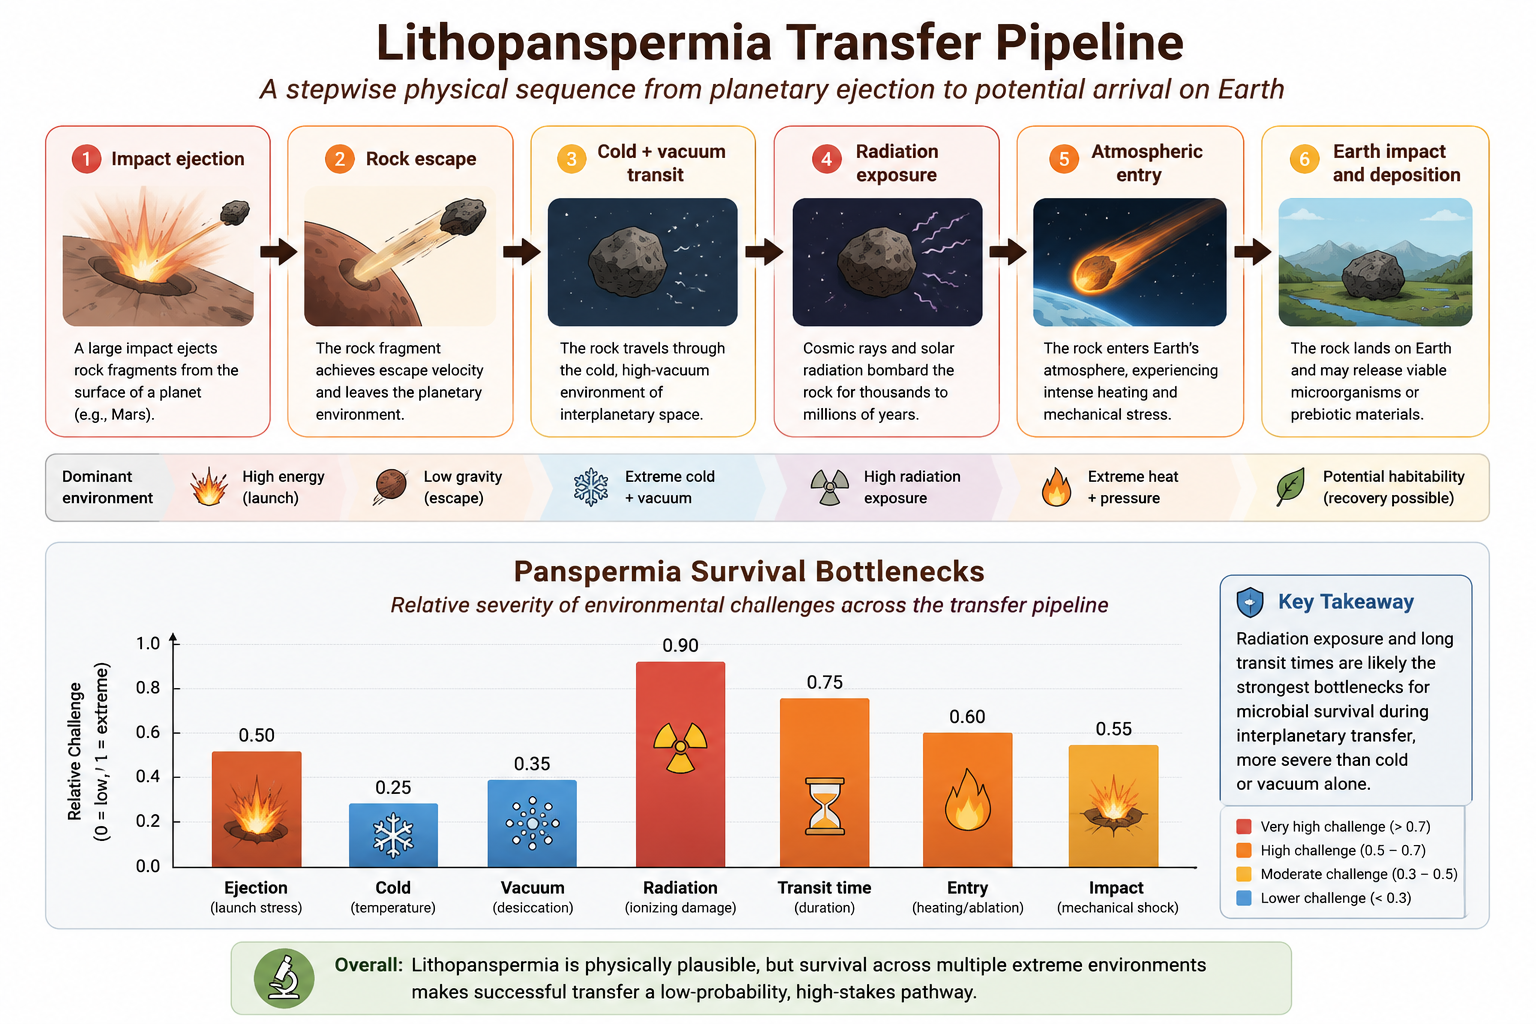
\includegraphics[width=1\linewidth]{figures/10_panspermia_transfer_pipeline} \caption{Integrated conceptual model of lithopanspermia showing the transfer sequence from planetary ejection to Earth arrival, along with the major environmental bottlenecks affecting microbial survival.}\label{fig:panspermia-pipeline}
\end{figure}

The upper portion of the figure illustrates the physical transfer pathway from planetary impact ejection to eventual arrival on Earth. The lower portion evaluates the relative severity of the environmental stresses encountered during this process.

Radiation exposure and long transit durations appear to represent the strongest survival bottlenecks, whereas cold alone may be less destructive for dormant microorganisms.

The figure also highlights an important conceptual distinction: panspermia primarily addresses the \textbf{transfer and survival} of life rather than the original emergence of life itself.

\section{What the Theory Explains Well}\label{what-the-theory-explains-well-7}

Panspermia theories are strongest at explaining:

\begin{itemize}
\tightlist
\item
  Interplanetary transfer of material
\item
  Possible dispersal of microorganisms
\item
  Distribution of organic compounds
\item
  Survival under extreme conditions
\item
  Potential continuity between planetary environments
\end{itemize}

The theory also provides a plausible explanation for why organic molecules are widespread throughout the Solar System.

\section{What Makes It Plausible}\label{what-makes-it-plausible-7}

Several observations support the plausibility of lithopanspermia:

\begin{itemize}
\tightlist
\item
  Meteorites from Mars have been found on Earth
\item
  Planetary impact ejecta are physically real
\item
  Organic molecules exist in meteorites and comets
\item
  Some microorganisms survive extreme radiation and vacuum
\item
  Dormant spores can remain viable for long periods
\end{itemize}

Laboratory studies demonstrate that certain extremophiles can tolerate conditions resembling portions of interplanetary space.

\section{Key Experimental and Observational Support}\label{key-experimental-and-observational-support-7}

Important supporting evidence includes:

\begin{itemize}
\tightlist
\item
  Discovery of Martian meteorites on Earth
\item
  Detection of amino acids in carbonaceous meteorites
\item
  Survival experiments involving bacterial spores
\item
  Space-exposure experiments on microorganisms
\item
  Observations of extremophiles in harsh terrestrial environments
\end{itemize}

Some microbial species have survived:

\begin{itemize}
\tightlist
\item
  Vacuum exposure
\item
  High radiation doses
\item
  Extreme cold
\item
  Desiccation
\item
  Extended dormancy
\end{itemize}

These findings significantly strengthened scientific interest in lithopanspermia as a physically plausible transport mechanism.

\section{Relationship to Other Origin-of-Life Theories}\label{relationship-to-other-origin-of-life-theories-1}

Panspermia differs fundamentally from most origin-of-life theories because it primarily addresses transfer rather than origin.

However, it can still interact with other theories:

\begin{itemize}
\tightlist
\item
  Primordial soup chemistry may occur on the source planet
\item
  Hydrothermal vent systems may support transferred organisms
\item
  RNA-world chemistry may still be required after transfer
\item
  Protocell and lipid-world mechanisms remain relevant
\end{itemize}

For this reason, panspermia is often treated as complementary rather than competitive with abiogenesis theories.

\section{Systems Perspective}\label{systems-perspective-7}

Within the broader comparative framework of this book, panspermia shifts the location of prebiotic evolution rather than eliminating the need for abiogenesis.

Even if life arrived from elsewhere, the original emergence of hereditary and evolving systems must still have occurred under suitable environmental conditions at some earlier location.

Thus, panspermia may help explain:

\begin{itemize}
\tightlist
\item
  Distribution of life
\item
  Spread of organics
\item
  Interplanetary biological exchange
\end{itemize}

but it does not independently explain the original emergence of heredity, metabolism, or Darwinian evolution.

\section{Major Gaps and Critiques}\label{major-gaps-and-critiques-7}

The principal criticism of panspermia is that it relocates rather than solves the origin-of-life problem.

Major unresolved questions include:

\begin{itemize}
\tightlist
\item
  Where did life originally emerge?
\item
  How likely is long-term survival during transit?
\item
  Can microorganisms survive millions of years in space?
\item
  How common are successful transfer pathways?
\end{itemize}

Directed panspermia introduces additional scientific and philosophical complications because it requires pre-existing intelligent life elsewhere.

\section{Current Scientific Standing}\label{current-scientific-standing-7}

Panspermia remains scientifically plausible as a transfer hypothesis, particularly in its lithopanspermia form.

However, it is generally not treated as a complete explanation for abiogenesis because it does not explain how life originally emerged.

Most modern researchers therefore view panspermia as:

\begin{itemize}
\tightlist
\item
  A plausible secondary mechanism
\item
  Potentially important for planetary exchange
\item
  Relevant to astrobiology
\item
  Complementary to abiogenesis theories rather than a replacement for them
\end{itemize}

\section{Comparative Assessment}\label{comparative-assessment-7}

\begin{longtable}[]{@{}ll@{}}
\toprule\noalign{}
Dimension & Assessment \\
\midrule\noalign{}
\endhead
\bottomrule\noalign{}
\endlastfoot
Primary Contribution & Interplanetary transfer and survival \\
Explanatory Strength & Strong for transfer, weak for origin \\
Mechanistic Plausibility & Moderate \\
Experimental Support & Moderate \\
Environmental Realism & Moderate \\
Main Limitation & Does not explain original abiogenesis \\
Integrative Potential & Moderate-High \\
Current Scientific Standing & Plausible but secondary \\
\end{longtable}

\section{Performance Across Major Abiogenesis Challenges}\label{performance-across-major-abiogenesis-challenges-1}

Table \ref{tab:panspermia-performance} summarizes how panspermia theories perform across major origin-of-life transitions.

\begin{table}

\caption{\label{tab:panspermia-performance}Comparative performance of Panspermia and Lithopanspermia theories across major abiogenesis challenges.}
\centering
\begin{tabular}[t]{l|l}
\hline
Challenge & Performance\\
\hline
Abiotic synthesis & Weak\\
\hline
Organic transfer & Strong\\
\hline
Molecular survival & Moderate-Strong\\
\hline
Catalysis & Weak\\
\hline
Compartment formation & Weak\\
\hline
Information storage & Weak\\
\hline
Hereditary replication & Weak\\
\hline
Darwinian evolution & Limited\\
\hline
\end{tabular}
\end{table}

Panspermia performs strongly as a transport and survival framework, but weakly as a standalone explanation for the original emergence of life.

\chapter{Comparative Synthesis}\label{comparative-synthesis}

\section{Chapter Overview}\label{chapter-overview-8}

No single origin-of-life theory currently explains all major transitions required for the emergence of living systems. Instead, modern origin-of-life research increasingly suggests that different theories may explain different stages of a broader transition from geochemistry to biology.

This final chapter synthesizes the major theories discussed throughout the book and compares their explanatory strengths, mechanistic focus, empirical support, and remaining limitations.

Rather than treating the theories as entirely competing alternatives, this comparative framework evaluates how they may interact within broader hybrid or sequential models of abiogenesis.

\section{Integrative Perspective}\label{integrative-perspective}

The origin of life likely required multiple major transitions occurring across different physical and chemical environments. These transitions include:

\begin{enumerate}
\def\labelenumi{\arabic{enumi}.}
\tightlist
\item
  Abiotic synthesis of organic molecules
\item
  Molecular concentration and organization
\item
  Polymerization and catalytic complexity
\item
  Emergence of information storage and replication
\item
  Formation of compartments and protocells
\item
  Development of energy transduction systems
\item
  Transition to Darwinian evolution
\end{enumerate}

Different theories appear strongest at explaining different portions of this sequence.

For example:

\begin{itemize}
\tightlist
\item
  Primordial soup models explain organic precursor synthesis
\item
  Wet--dry cycles and clay surfaces support polymerization
\item
  RNA World addresses heredity and replication
\item
  Metabolism-first models explain energy flow and catalytic organization
\item
  Lipid-world theories explain compartment formation
\item
  Panspermia addresses interplanetary transfer and survival
\end{itemize}

This broader systems perspective suggests that abiogenesis may not have followed a single isolated pathway.

\section{Comparative Framework}\label{comparative-framework}

Throughout this book, each theory has been evaluated using several recurring criteria:

\begin{itemize}
\tightlist
\item
  Explanatory scope
\item
  Mechanistic plausibility
\item
  Experimental support
\item
  Environmental realism
\item
  Integration with other models
\item
  Remaining scientific gaps
\item
  Capacity to support Darwinian evolution
\end{itemize}

Figure \ref{fig:comparative-matrix} summarizes how the major theories compare across key origin-of-life problem domains.

\begin{figure}
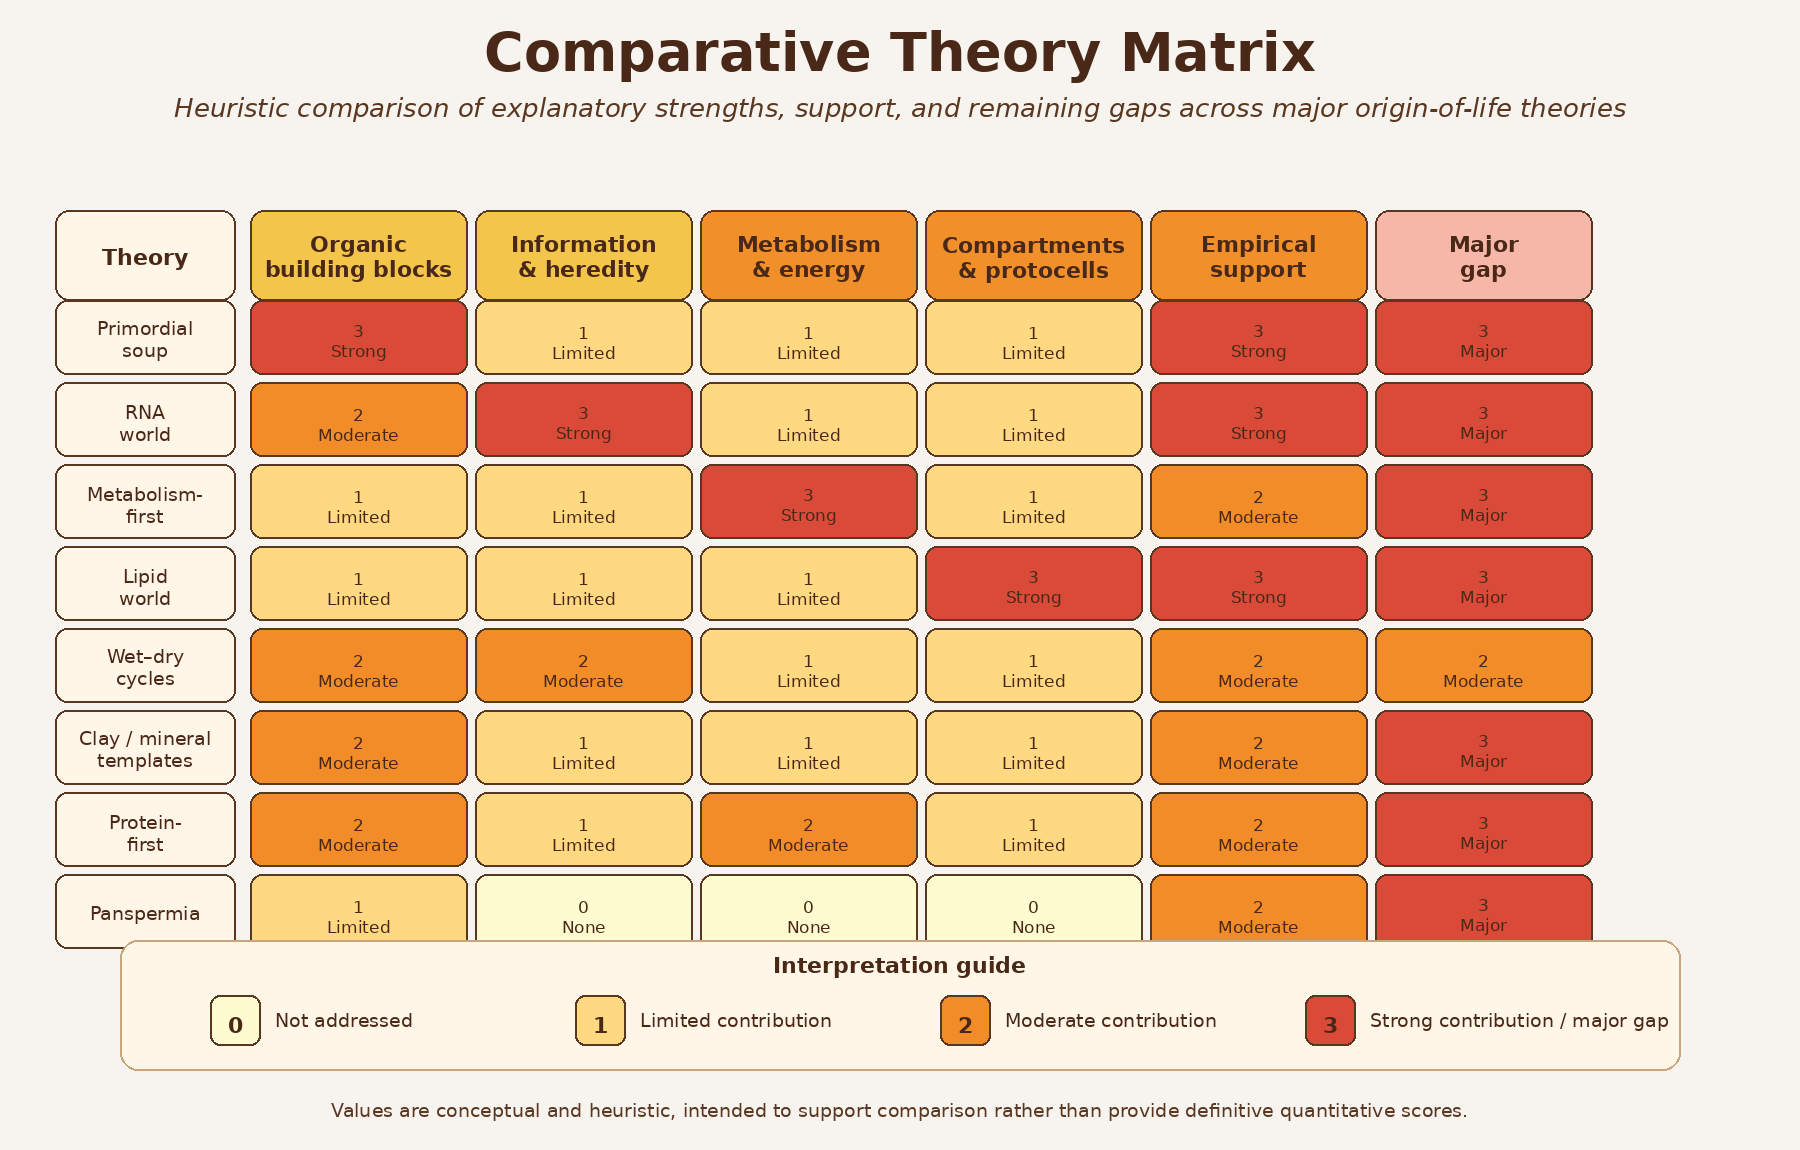
\includegraphics[width=1\linewidth]{figures/11_comparative_theory_matrix} \caption{Comparative matrix showing how major origin-of-life theories address different stages and challenges in the transition from chemistry to early life.}\label{fig:comparative-matrix}
\end{figure}

The figure illustrates an important conclusion emerging from modern origin-of-life research: most theories are strongest within a limited explanatory domain rather than across the entire origin sequence.

For example:

\begin{itemize}
\tightlist
\item
  \textbf{Primordial soup} performs strongly in abiotic synthesis but weakly in heredity
\item
  \textbf{RNA World} is powerful for information storage and replication but weaker for prebiotic accessibility
\item
  \textbf{Metabolism-first theories} explain energy flow and catalytic continuity but not encoded heredity
\item
  \textbf{Lipid-world theories} solve compartmentalization problems but not replication
\item
  \textbf{Clay/mineral models} support molecular organization and templating
\item
  \textbf{Wet--dry cycle theories} explain concentration and polymerization dynamics
\item
  \textbf{Protein-first models} emphasize primitive catalysis
\item
  \textbf{Panspermia} addresses transfer rather than original emergence
\end{itemize}

This comparative structure reinforces the broader conclusion that no current theory independently explains all major abiogenesis transitions.

\section{Empirical Support and Explanatory Scope}\label{empirical-support-and-explanatory-scope}

Theories differ not only in what they explain, but also in the degree of empirical support available for their central mechanisms.

Figure \ref{fig:evidence-scope} compares major theories according to two broad dimensions:

\begin{enumerate}
\def\labelenumi{\arabic{enumi}.}
\tightlist
\item
  Relative empirical support
\item
  Relative explanatory scope
\end{enumerate}

\begin{figure}

\includegraphics[width=0.9\linewidth]{figures/12_evidence_vs_scope_matrix} \caption{Conceptual comparison of relative empirical support and explanatory scope among major origin-of-life theories.}\label{fig:evidence-scope}
\end{figure}

The figure highlights several important patterns:

\begin{itemize}
\tightlist
\item
  Some theories possess strong empirical support but narrow explanatory scope
\item
  Others provide broad conceptual frameworks but remain experimentally difficult to validate
\item
  Several theories occupy complementary rather than competing positions
\end{itemize}

For example:

\begin{itemize}
\tightlist
\item
  Primordial soup chemistry has substantial experimental support
\item
  RNA catalysis is strongly supported experimentally
\item
  Hydrothermal vent models are geochemically plausible
\item
  Lipid vesicle self-assembly is experimentally reproducible
\item
  Panspermia is physically plausible but does not address abiogenesis itself
\end{itemize}

At the same time, major unresolved problems remain across all theories, particularly regarding:

\begin{itemize}
\tightlist
\item
  Transition from chemistry to heredity
\item
  Emergence of encoded information
\item
  Origin of self-sustaining replication
\item
  Integration of metabolism with compartments
\item
  Transition to Darwinian evolution
\end{itemize}

\section{Hybrid and Sequential Models}\label{hybrid-and-sequential-models}

Increasingly, modern research favors hybrid or sequential models that combine mechanisms from multiple theories.

Possible integrated scenarios include:

\begin{itemize}
\tightlist
\item
  Primordial synthesis of organics in atmospheric or hydrothermal settings
\item
  Concentration through evaporation, mineral surfaces, or porous vents
\item
  Polymerization assisted by wet--dry cycles or mineral templating
\item
  Emergence of catalytic RNA or peptide networks
\item
  Encapsulation within lipid vesicles
\item
  Coupling of metabolism, heredity, and compartmentalization
\item
  Gradual transition to cellular evolution
\end{itemize}

Under this view, different theories may describe different stages within a larger evolutionary continuum.

Rather than asking which theory is entirely correct, current research increasingly asks:

\begin{quote}
Which combinations of mechanisms could realistically cooperate under early Earth conditions?
\end{quote}

This systems-level perspective represents a major shift in modern origin-of-life research.

\section{Remaining Grand Challenges}\label{remaining-grand-challenges}

Despite major advances, several fundamental questions remain unresolved.

\subsection{1. Origin of Heredity}\label{origin-of-heredity}

No theory fully explains how stable, self-replicating informational systems first emerged under realistic prebiotic conditions.

\subsection{2. Integration Problem}\label{integration-problem}

Individual components of life---metabolism, heredity, and compartments---must ultimately become integrated into unified evolving systems.

\subsection{3. Environmental Uncertainty}\label{environmental-uncertainty}

The precise environmental conditions of early Earth remain incompletely understood, including:

\begin{itemize}
\tightlist
\item
  Atmospheric composition
\item
  Ocean chemistry
\item
  Temperature regimes
\item
  Availability of catalytic minerals
\item
  Stability of surface environments
\end{itemize}

\subsection{4. Transition to Darwinian Evolution}\label{transition-to-darwinian-evolution}

A major unresolved challenge is understanding how non-living chemistry crossed the threshold into open-ended biological evolution.

\section{Broader Scientific Importance}\label{broader-scientific-importance}

Origin-of-life research extends beyond explaining early Earth alone.

The field also informs:

\begin{itemize}
\tightlist
\item
  Astrobiology
\item
  Exoplanet habitability
\item
  Planetary evolution
\item
  Systems chemistry
\item
  Synthetic biology
\item
  Search for extraterrestrial life
\end{itemize}

Understanding abiogenesis may therefore help answer broader questions concerning:

\begin{itemize}
\tightlist
\item
  Whether life is rare or common in the universe
\item
  Which planetary environments are potentially habitable
\item
  How biological complexity emerges from chemistry
\end{itemize}

\section{Limitations of Comparative Framing}\label{limitations-of-comparative-framing}

The comparative figures presented in this chapter are conceptual rather than strictly quantitative.

Their rankings are heuristic and intended to support structured scientific comparison rather than definitive scoring.

Several important limitations should be acknowledged:

\begin{itemize}
\tightlist
\item
  Empirical support varies across subdomains
\item
  Some theories remain highly speculative
\item
  New experimental discoveries may substantially alter current interpretations
\item
  Theories overlap and interact in complex ways
\item
  Abiogenesis may not follow a single universal pathway
\end{itemize}

Accordingly, the figures should be interpreted as conceptual synthesis tools rather than final scientific conclusions.

\section{Final Perspective}\label{final-perspective}

The origin of life remains one of the most difficult and interdisciplinary problems in science.

Current evidence suggests that no single theory completely explains the transition from abiotic chemistry to evolving cellular life. Instead, the emergence of life likely involved multiple interacting processes operating across different environments and timescales.

Theories once viewed as competing alternatives increasingly appear capable of contributing complementary pieces to a larger systems-level explanation.

In this sense, the origin of life may ultimately be understood not as a single event, but as a progressive transition from geochemistry to biological complexity through the interaction of many partially understood mechanisms.

\chapter{Research Directions and Integrative Models}\label{research-directions-and-integrative-models}

\section{Moving Beyond Single-Theory Explanations}\label{moving-beyond-single-theory-explanations}

Modern origin-of-life research increasingly emphasizes integrative and multi-stage models rather than treating individual theories as complete standalone explanations.

Early origin-of-life research often focused on identifying a single dominant mechanism responsible for the emergence of life. However, contemporary research increasingly suggests that different theories may explain different stages within a broader transition from geochemistry to biology.

For example:

\begin{itemize}
\tightlist
\item
  Primordial soup models help explain the abiotic formation of organic building blocks.
\item
  Wet--dry cycle and clay-template models help explain concentration and polymerization processes.
\item
  Metabolism-first theories address energy flow and catalytic organization.
\item
  RNA World models focus on heredity and molecular evolution.
\item
  Lipid World theories help explain compartment formation and protocell development.
\end{itemize}

Rather than competing as mutually exclusive explanations, these mechanisms may have interacted sequentially or simultaneously within early Earth environments.

\section{Hybrid and Coupled Mechanisms}\label{hybrid-and-coupled-mechanisms}

A major direction in modern research is understanding how these mechanisms could have coupled together under realistic planetary conditions.

Current studies investigate questions such as:

\begin{itemize}
\tightlist
\item
  How were organic molecules concentrated in early environments?
\item
  How did catalytic surfaces promote polymer formation?
\item
  How were primitive metabolic reactions sustained?
\item
  How did informational molecules emerge and persist?
\item
  How were early reaction systems compartmentalized within protocells?
\item
  How did prebiotic systems transition into Darwinian evolution?
\end{itemize}

This systems-level perspective treats abiogenesis as a progressive sequence of interacting transitions rather than a single isolated event.

\section{Experimental and Computational Advances}\label{experimental-and-computational-advances}

Recent advances in experimental chemistry, planetary science, systems chemistry, molecular evolution, and computational modeling have significantly expanded the field.

Modern origin-of-life research now combines:
- laboratory simulations,
- microfluidic experiments,
- mineral-surface chemistry,
- RNA evolution studies,
- protocell engineering,
- planetary environment modeling,
- and computational network analysis.

These approaches allow researchers to evaluate which combinations of mechanisms remain chemically and physically plausible under early Earth conditions.

\section{Remaining Challenges}\label{remaining-challenges}

Despite major progress, several fundamental questions remain unresolved:

\begin{itemize}
\tightlist
\item
  How did heredity emerge from non-living chemistry?
\item
  How were stable self-replicating systems established?
\item
  How did metabolism, replication, and compartmentalization become integrated?
\item
  What environmental settings were most favorable for these transitions?
\item
  Did life emerge once or multiple times?
\item
  Could similar processes occur elsewhere in the universe?
\end{itemize}

No current theory fully explains the complete transition from geochemistry to cellular life.

\section{Final Perspective}\label{final-perspective-1}

The modern scientific view increasingly treats abiogenesis as a multi-step planetary process involving interacting chemical, physical, and evolutionary transitions.

As a result, the central question is no longer simply \emph{which individual theory is correct}, but rather:

\begin{quote}
\emph{How did multiple complementary mechanisms interact to produce the emergence of early cellular life?}
\end{quote}

This integrative perspective represents one of the most important shifts in contemporary origin-of-life research and continues to guide future experimental and theoretical work.

\chapter*{References}\label{references}
\addcontentsline{toc}{chapter}{References}

This section lists several foundational and influential works related to origin-of-life research, including historical theories, modern reviews, experimental studies, and astrobiology perspectives. The references cited throughout the book are automatically generated below.

\section{Foundational Works}\label{foundational-works}

The modern scientific study of abiogenesis emerged from early twentieth-century attempts to explain how non-living chemistry could transition into biological systems. Important foundational contributions include the primordial soup hypothesis proposed by Oparin and Haldane, the landmark experiments of Miller and Urey, and later developments involving molecular evolution, catalysis, and RNA-based heredity.

Several foundational ideas shaped the development of modern origin-of-life research:

\begin{itemize}
\tightlist
\item
  \emph{Chemical evolution frameworks} proposed by Oparin and Haldane
\item
  \emph{Prebiotic synthesis experiments} demonstrated by Miller and Urey
\item
  \emph{Molecular evolution models} developed by Eigen
\item
  \emph{RNA World concepts} introduced by Gilbert
\item
  \emph{Metabolism-first theories} proposed by Wächtershäuser
\item
  \emph{Hydrothermal vent hypotheses} advanced by Martin and Russell
\end{itemize}

Together, these works established the conceptual foundations for modern abiogenesis research and continue to influence contemporary integrative models.

\section{Modern Reviews}\label{modern-reviews}

Modern origin-of-life research has increasingly shifted toward interdisciplinary and integrative approaches that combine geochemistry, molecular biology, systems chemistry, planetary science, and computational modeling.

Contemporary review literature commonly focuses on several major research themes:

\begin{itemize}
\tightlist
\item
  \emph{Prebiotic chemistry and organic synthesis}
\item
  \emph{Self-organization and chemical complexity}
\item
  \emph{RNA catalysis and molecular heredity}
\item
  \emph{Lipid vesicles and protocell formation}
\item
  \emph{Hydrothermal vent and metabolism-first systems}
\item
  \emph{Wet--dry cycling and environmental concentration mechanisms}
\item
  \emph{Systems-level and network-based models of abiogenesis}
\item
  \emph{Astrobiology and planetary habitability}
\end{itemize}

A major conclusion emerging from modern reviews is that no single theory currently explains all major transitions required for the emergence of life. Instead, many researchers now view abiogenesis as a multi-stage process involving interacting mechanisms operating across different environmental and chemical contexts.

As a result, contemporary origin-of-life research increasingly emphasizes hybrid and integrative frameworks that connect prebiotic synthesis, catalysis, compartment formation, energy flow, and molecular evolution into broader transition models.

\section{Experimental Studies}\label{experimental-studies}

Experimental origin-of-life research investigates whether biologically relevant molecules, structures, and processes can emerge under plausible prebiotic conditions.

Modern laboratory research explores several major experimental directions:

\begin{itemize}
\tightlist
\item
  \emph{Abiotic amino acid and organic molecule synthesis}
\item
  \emph{Prebiotic nucleotide and RNA precursor formation}
\item
  \emph{Wet--dry cycle polymerization and concentration mechanisms}
\item
  \emph{Ribozyme activity and molecular evolution experiments}
\item
  \emph{Lipid vesicle self-assembly and protocell formation}
\item
  \emph{Mineral-surface adsorption and catalytic templating}
\item
  \emph{Hydrothermal vent and geochemical reactor simulations}
\item
  \emph{Autocatalytic and systems-chemistry networks}
\end{itemize}

These experiments aim to determine whether key biological transitions could arise naturally from physical and chemical processes operating on the early Earth.

Modern experimental approaches increasingly integrate environmental cycling, systems chemistry, synthetic protocells, microfluidic reactors, and computational modeling to investigate how multiple prebiotic mechanisms may have interacted simultaneously rather than independently.

Although no experiment has yet recreated the complete transition from chemistry to life, experimental studies continue to provide important constraints on plausibility, environmental conditions, and potential transition pathways.

\section{Astrobiology and Panspermia}\label{astrobiology-and-panspermia}

Astrobiology expands origin-of-life research beyond Earth by examining planetary habitability, organic chemistry in space, and the possibility of interplanetary transfer of biological material.

Research in this area investigates several major themes:

\begin{itemize}
\tightlist
\item
  \emph{Organic molecules in meteorites and interstellar environments}
\item
  \emph{Mars--Earth rock transfer and impact ejection dynamics}
\item
  \emph{Microbial survival under radiation, vacuum, and extreme cold}
\item
  \emph{Exoplanet habitability and planetary environments}
\item
  \emph{Cometary and asteroid delivery of prebiotic compounds}
\item
  \emph{Lithopanspermia transfer and survivability models}
\item
  \emph{Planetary protection and contamination studies}
\end{itemize}

Astrobiological research demonstrates that many organic molecules relevant to life can form naturally in extraterrestrial environments and may have been delivered to the early Earth through meteorites, comets, and planetary impacts.

Although panspermia does not explain the ultimate origin of life itself, it remains scientifically important as a transfer and survivability hypothesis. In particular, lithopanspermia reframes the problem as a sequence of physical survival stages involving ejection, space transit, radiation exposure, atmospheric entry, and planetary deposition.

As a result, astrobiology broadens the study of abiogenesis from a strictly Earth-based problem into a larger planetary and cosmic context.

\chapter{Selected Bibliography}\label{selected-bibliography}

Arrhenius, S. (1908). \emph{Worlds in the Making: The Evolution of the Universe}. Harper \& Brothers.

Crick, F. H. C., \& Orgel, L. E. (1973). Directed panspermia. \emph{Icarus, 19}(3), 341--346.

Deamer, D. (2012). \emph{First Life: Discovering the Connections between Stars, Cells, and How Life Began}. University of California Press.

Eigen, M. (1971). Selforganization of matter and the evolution of biological macromolecules. \emph{Naturwissenschaften, 58}, 465--523.

Ferris, J. P. (2006). Montmorillonite-catalysed formation of RNA oligomers: The possible role of catalysis in the origins of life. \emph{Philosophical Transactions of the Royal Society B, 361}(1474), 1777--1786.

Gilbert, W. (1986). The RNA world. \emph{Nature, 319}(6055), 618.

Haldane, J. B. S. (1929). The origin of life. \emph{The Rationalist Annual}, 148, 3--10.

Joyce, G. F. (2002). The antiquity of RNA-based evolution. \emph{Nature, 418}(6894), 214--221.

Martin, W., \& Russell, M. J. (2007). On the origin of biochemistry at an alkaline hydrothermal vent. \emph{Philosophical Transactions of the Royal Society B, 362}(1486), 1887--1925.

Miller, S. L. (1953). A production of amino acids under possible primitive Earth conditions. \emph{Science, 117}(3046), 528--529.

Oparin, A. I. (1938). \emph{The Origin of Life}. Macmillan.

Wächtershäuser, G. (1988). Before enzymes and templates: Theory of surface metabolism. \emph{Microbiological Reviews, 52}(4), 452--484.

\section{Complete Reference List}\label{complete-reference-list}

The complete bibliography for all in-text citations used throughout the book is automatically generated below.

\phantomsection\label{refs}
\begin{CSLReferences}{1}{0}
\bibitem[\citeproctext]{ref-arrhenius1908}
Arrhenius, Svante. 1908. {``Worlds in the Making.''}

\bibitem[\citeproctext]{ref-crick1973}
Crick, Francis, and Leslie Orgel. 1973. {``Directed Panspermia.''} \emph{Icarus} 19: 341--46.

\bibitem[\citeproctext]{ref-deamer2012}
Deamer, David. 2012. {``First Life: Discovering the Connections Between Stars, Cells, and How Life Began.''}

\bibitem[\citeproctext]{ref-ferris2006}
Ferris, James P. 2006. {``Montmorillonite-Catalysed Formation of RNA Oligomers.''} \emph{Philosophical Transactions of the Royal Society B} 361: 1777--86.

\bibitem[\citeproctext]{ref-gilbert1986}
Gilbert, Walter. 1986. {``The RNA World.''} \emph{Nature} 319: 618.

\bibitem[\citeproctext]{ref-joyce2002}
Joyce, Gerald F. 2002. {``The Antiquity of RNA-Based Evolution.''} \emph{Nature} 418: 214--21.

\bibitem[\citeproctext]{ref-martin2008}
Martin, William, John Baross, Deborah Kelley, and Michael J. Russell. 2008. {``Hydrothermal Vents and the Origin of Life.''} \emph{Nature Reviews Microbiology} 6: 805--14.

\bibitem[\citeproctext]{ref-miller1953}
Miller, Stanley L. 1953. {``A Production of Amino Acids Under Possible Primitive Earth Conditions.''} \emph{Science} 117: 528--29.

\bibitem[\citeproctext]{ref-wachtershauser1988}
Wächtershäuser, Günter. 1988. {``Before Enzymes and Templates: Theory of Surface Metabolism.''} \emph{Microbiological Reviews} 52: 452--84.

\end{CSLReferences}

\end{document}
